\documentclass{article}
\usepackage{geometry}
\usepackage{amsmath}
\usepackage{lscape}
\geometry{verbose,tmargin=2.5cm,bmargin=2.5cm,lmargin=2.5cm,rmargin=2.5cm}

\begin{document}



\title{SIS NMF Final: Diagnosis to DSD}
\maketitle

%%%%%%%%%%%%%%%%%%%%%%%%%%%%%%%%%%%%%%%%%%%%%%%%%%%%%%%%%%%%%%%%%%%%%%
% LIBRARIES
%%%%%%%%%%%%%%%%%%%%%%%%%%%%%%%%%%%%%%%%%%%%%%%%%%%%%%%%%%%%%%%%%%%%%%
\section{Preparation}
\begin{knitrout}
\definecolor{shadecolor}{rgb}{0.969, 0.969, 0.969}\color{fgcolor}\begin{kframe}
\begin{alltt}
\hlkwd{options}\hlstd{(}\hlkwc{java.parameters} \hlstd{=} \hlstr{"-Xmx4G"}\hlstd{)}

\hlkwd{library}\hlstd{(survival)}
\end{alltt}


{\ttfamily\noindent\itshape\color{messagecolor}{\#\# Loading required package: splines}}\begin{alltt}
\hlkwd{library}\hlstd{(energy)}
\hlkwd{library}\hlstd{(NMF)}
\end{alltt}


{\ttfamily\noindent\itshape\color{messagecolor}{\#\# Loading required package: pkgmaker\\\#\# Loading required package: registry\\\#\# Loading required package: rngtools\\\#\# Loading required package: cluster\\\#\# NMF - BioConductor layer [OK] | Shared memory capabilities [OK] | Cores 7/8}}\begin{alltt}
\hlkwd{library}\hlstd{(nnls)}

\hlkwd{library}\hlstd{(bnlearn)}
\end{alltt}


{\ttfamily\noindent\itshape\color{messagecolor}{\#\# \\\#\# Attaching package: 'bnlearn'\\\#\# \\\#\# The following object is masked from 'package:NMF':\\\#\# \\\#\#\ \ \ \  compare}}\begin{alltt}
\hlkwd{library}\hlstd{(glmulti)}
\end{alltt}


{\ttfamily\noindent\itshape\color{messagecolor}{\#\# Loading required package: rJava\\\#\# \\\#\# Attaching package: 'glmulti'\\\#\# \\\#\# The following object is masked from 'package:NMF':\\\#\# \\\#\#\ \ \ \  consensus}}\begin{alltt}
\hlkwd{library}\hlstd{(glmnet)}
\end{alltt}


{\ttfamily\noindent\itshape\color{messagecolor}{\#\# Loading required package: Matrix\\\#\# Loaded glmnet 1.9-8}}\begin{alltt}
\hlkwd{library}\hlstd{(RColorBrewer)}
\hlkwd{library}\hlstd{(gplots)}
\end{alltt}


{\ttfamily\noindent\itshape\color{messagecolor}{\#\# \\\#\# Attaching package: 'gplots'\\\#\# \\\#\# The following object is masked from 'package:stats':\\\#\# \\\#\#\ \ \ \  lowess}}\begin{alltt}
\hlkwd{library}\hlstd{(xtable)}
\hlkwd{library}\hlstd{(stargazer)}
\end{alltt}


{\ttfamily\noindent\itshape\color{messagecolor}{\#\# \\\#\# Please cite as: \\\#\# \\\#\#\ \ Hlavac, Marek (2014). stargazer: LaTeX code and ASCII text for well-formatted regression and summary statistics tables.\\\#\#\ \ R package version 5.1. http://CRAN.R-project.org/package=stargazer}}\begin{alltt}
\hlkwd{load}\hlstd{(}\hlstr{"image.rda"}\hlstd{)}
\end{alltt}
\end{kframe}
\end{knitrout}


%%%%%%%%%%%%%%%%%%%%%%%%%%%%%%%%%%%%%%%%%%%%%%%%%%%%%%%%%%%%%%%%%%%%%%
% COHORT CHARACTERISTICS
%%%%%%%%%%%%%%%%%%%%%%%%%%%%%%%%%%%%%%%%%%%%%%%%%%%%%%%%%%%%%%%%%%%%%%
\section{Cohort characteristics}
\begin{knitrout}
\definecolor{shadecolor}{rgb}{0.969, 0.969, 0.969}\color{fgcolor}\begin{kframe}
\begin{alltt}
\hlstd{cpvs.diag_dsd}\hlopt{$}\hlstd{Path.TumourLocation[cpvs.diag_dsd}\hlopt{$}\hlstd{Path.TumourLocation} \hlopt{==} \hlstr{""}\hlstd{]} \hlkwb{=} \hlnum{NA}
\hlstd{cpvs.diag_dsd}\hlopt{$}\hlstd{Path.Nodes.Regional.Involved.Fraction} \hlkwb{=} \hlstd{cpvs.diag_dsd}\hlopt{$}\hlstd{Path.Nodes.Regional.Involved} \hlopt{/} \hlstd{cpvs.diag_dsd}\hlopt{$}\hlstd{Path.Nodes.Regional.Total}
\hlstd{cpvs.diag_dsd}\hlopt{$}\hlstd{Treat.Surgery.ExcisionStatus.Coarse} \hlkwb{=} \hlkwd{ordered}\hlstd{(}\hlkwd{ifelse}\hlstd{(cpvs.diag_dsd}\hlopt{$}\hlstd{Treat.Surgery.ExcisionStatus} \hlopt{==} \hlstr{"R0"}\hlstd{,} \hlstr{"Clear"}\hlstd{,} \hlstr{"Involved"}\hlstd{),} \hlkwc{levels} \hlstd{=} \hlkwd{c}\hlstd{(}\hlstr{"Clear"}\hlstd{,} \hlstr{"Involved"}\hlstd{))}
\hlstd{cpvs.diag_dsd}\hlopt{$}\hlstd{Path.Grade.Coarse} \hlkwb{=} \hlkwd{ordered}\hlstd{(}\hlkwd{ifelse}\hlstd{(cpvs.diag_dsd}\hlopt{$}\hlstd{Path.Grade} \hlopt \hlkwd{c}\hlstd{(}\hlstr{"1"}\hlstd{,} \hlstr{"2"}\hlstd{),} \hlstr{"1or2"}\hlstd{,} \hlstr{"3or4"}\hlstd{),} \hlkwc{levels} \hlstd{=} \hlkwd{c}\hlstd{(}\hlstr{"1or2"}\hlstd{,} \hlstr{"3or4"}\hlstd{))}
\hlstd{cpvs.diag_dsd}\hlopt{$}\hlstd{Path.TumourLocation.Coarse} \hlkwb{=} \hlkwd{factor}\hlstd{(}\hlkwd{ifelse}\hlstd{(cpvs.diag_dsd}\hlopt{$}\hlstd{Path.TumourLocation} \hlopt \hlkwd{c}\hlstd{(}\hlstr{"Head"}\hlstd{,} \hlstr{"Head (Uncinate)"}\hlstd{),} \hlstr{"Head"}\hlstd{,} \hlstr{"Other"}\hlstd{))}

\hlkwd{summary}\hlstd{(cpvs.diag_dsd)}
\end{alltt}
\begin{verbatim}
##   Patient.ID        Patient.Gender                      Patient.Ethnicity
##  Length:110         Female:50      Asian                         :  5    
##  Class :character   Male  :60      Asian, White/Caucasian        :  0    
##  Mode  :character                  Black/African                 :  0    
##                                    Black/African, White/Caucasian:  0    
##                                    White/Caucasian               :104    
##                                    NA's                          :  1    
##                                                                          
##                  Patient.Country History.LastFollowup.Date
##  Australia               :110    Min.   :2007-06-29       
##  Italy                   :  0    1st Qu.:2011-08-19       
##  New Zealand             :  0    Median :2013-03-12       
##  Puerto Rico             :  0    Mean   :2012-10-16       
##  United Kingdom          :  0    3rd Qu.:2014-04-24       
##  United States of America:  0    Max.   :2014-09-23       
##                                  NA's   :1                
##  History.Smoking.PackYears History.Diagnosis.Date
##  Min.   : 0.75             Min.   :2007-06-04    
##  1st Qu.: 9.00             1st Qu.:2010-01-28    
##  Median :22.50             Median :2011-01-04    
##  Mean   :26.89             Mean   :2011-01-14    
##  3rd Qu.:43.75             3rd Qu.:2012-02-15    
##  Max.   :70.00             Max.   :2012-10-17    
##  NA's   :68                                      
##  History.Diagnosis.AgeAtYears History.Surgery.Date
##  Min.   :36.0                 Min.   :2007-05-29  
##  1st Qu.:61.0                 1st Qu.:2010-01-22  
##  Median :67.0                 Median :2011-01-01  
##  Mean   :66.4                 Mean   :2011-01-13  
##  3rd Qu.:73.0                 3rd Qu.:2012-02-13  
##  Max.   :87.0                 Max.   :2012-10-17  
##                                                   
##                                            Treat.Surgery.Procedure
##  Classic Whipple                                       :79        
##  Splenectomy, Subtotal Panc/L sided Panc or distal Panc: 6        
##  Cholecystectomy, Classic Whipple                      : 5        
##  Subtotal Panc/L sided Panc or distal Panc             : 4        
##  Classic Whipple, Exploratory laparotomy               : 3        
##  PPPD                                                  : 3        
##  (Other)                                               :10        
##  Treat.Surgery.ExcisionStatus Treat.Surgery.Margin.Pancreatic
##  R0:69                        <2 mm   : 4                    
##  R1:35                        Clear   :88                    
##  R2: 6                        Involved: 9                    
##                               NA's    : 9                    
##                                                              
##                                                              
##                                                              
##  Treat.Surgery.MarginSizeMm.Pancreatic Treat.Surgery.Margin.Periunc
##  Min.   : 0.0                          <2 mm   :20                 
##  1st Qu.: 5.0                          Clear   :52                 
##  Median :10.0                          Involved:15                 
##  Mean   :10.6                          NA's    :23                 
##  3rd Qu.:10.2                                                      
##  Max.   :40.0                                                      
##  NA's   :30                                                        
##  Treat.Surgery.MarginSizeMm.Periunc Treat.Surgery.Margin.PVGroove
##  Min.   : 0.00                      <2 mm   :23                  
##  1st Qu.: 1.00                      Clear   :55                  
##  Median : 3.00                      Involved:12                  
##  Mean   : 6.21                      NA's    :20                  
##  3rd Qu.:10.00                                                   
##  Max.   :40.00                                                   
##  NA's   :43                                                      
##  Treat.Surgery.MarginSizeMm.PVGroove Treat.Surgery.Margin.Retrop
##  Min.   : 0.00                       <2 mm   :21                
##  1st Qu.: 1.00                       Clear   :68                
##  Median : 3.00                       Involved: 9                
##  Mean   : 4.08                       NA's    :12                
##  3rd Qu.: 5.00                                                  
##  Max.   :30.00                                                  
##  NA's   :45                                                     
##  Treat.Surgery.MarginSizeMm.Retrop Treat.Surgery.Margin.CBD
##  Min.   : 0.10                     <2 mm   : 1             
##  1st Qu.: 1.75                     Clear   :83             
##  Median : 3.00                     Involved: 0             
##  Mean   : 5.62                     NA's    :26             
##  3rd Qu.:10.00                                             
##  Max.   :25.00                                             
##  NA's   :31                                                
##  Treat.Surgery.MarginSizeMm.CBD Treat.Surgery.Margin.Duodenal
##  Min.   : 1.0                   Clear   :60                  
##  1st Qu.:11.8                   Involved: 1                  
##  Median :20.0                   NA's    :49                  
##  Mean   :23.6                                                
##  3rd Qu.:32.5                                                
##  Max.   :55.0                                                
##  NA's   :47                                                  
##  Treat.Surgery.MarginSizeMm.Duodenal Treat.Surgery.Margin.Gastric
##  Min.   : 10.0                       Clear:59                    
##  1st Qu.: 40.0                       NA's :51                    
##  Median : 80.0                                                   
##  Mean   : 86.2                                                   
##  3rd Qu.:132.5                                                   
##  Max.   :190.0                                                   
##  NA's   :102                                                     
##  Treat.Surgery.MarginSizeMm.Gastric Treat.Surgery.Margin.Comments
##  Min.   : 10.0                      Length:110                   
##  1st Qu.: 50.0                      Class :character             
##  Median : 70.0                      Mode  :character             
##  Mean   : 67.9                                                   
##  3rd Qu.: 97.5                                                   
##  Max.   :100.0                                                   
##  NA's   :103                                                     
##                           Path.HistoType
##  Pancreatic Ductal Adenocarcinoma:110   
##  Acinar Cell Carcinoma           :  0   
##  Ampullary Adenocarcinoma        :  0   
##  Carcinoid Tumour                :  0   
##  Cholangiocarcinoma              :  0   
##  Clear Cell Carcinoma            :  0   
##  (Other)                         :  0   
##                    Path.HistoType.Subtype Path.Grade
##  Gastric                      : 0         1: 8      
##  Intestinal                   : 0         2:71      
##  Mixed                        : 0         3:30      
##  Not otherwise Specified (NOS):31         4: 1      
##  Pancreatobiliary             :13                   
##  Squamous                     : 0                   
##  NA's                         :66                   
##       Path.TumourLocation Path.TumourSizeMm Path.Invasion.PN
##  Head           :83       Min.   :10.0      Absent :13      
##  Head (Uncinate):10       1st Qu.:28.0      Present:96      
##  Tail           : 9       Median :35.0      NA's   : 1      
##  Body           : 7       Mean   :37.6                      
##                 : 0       3rd Qu.:45.0                      
##  (Other)        : 0       Max.   :90.0                      
##  NA's           : 1       NA's   :1                         
##  Path.Invasion.VS Path.Nodes.Regional.Total Path.Nodes.Regional.Involved
##  Absent :34       Min.   : 0.0              Min.   : 0.00               
##  Present:72       1st Qu.:11.0              1st Qu.: 1.00               
##  NA's   : 4       Median :16.0              Median : 2.00               
##                   Mean   :18.1              Mean   : 3.18               
##                   3rd Qu.:24.0              3rd Qu.: 4.00               
##                   Max.   :46.0              Max.   :18.00               
##                                                                         
##  Path.Nodes.SepRec.Total Path.Nodes.SepRec.Involved
##  Min.   : 0.0            Min.   : 0.00             
##  1st Qu.:11.0            1st Qu.: 1.00             
##  Median :16.0            Median : 2.00             
##  Mean   :18.1            Mean   : 3.18             
##  3rd Qu.:24.0            3rd Qu.: 4.00             
##  Max.   :46.0            Max.   :18.00             
##                                                    
##                                    Staging.Version Staging.pM Staging.pN
##  pTNM AJCC 6th Ed 2002                     :14     M0  :  2   N0  :25   
##  pTNM AJCC 7th Ed 2010                     :96     M1  :  6   N1  :84   
##  pTNM AJCC 7th Ed 2010 (Ampulla)           : 0     NA's:102   NA's: 1   
##  pTNM AJCC 7th Ed 2010 (Cholangiocarcinoma): 0                          
##  pTNM AJCC 7th Ed 2010 (Neuroendocrine)    : 0                          
##                                                                         
##                                                                         
##  Staging.pT Staging.Stage    History.Recurrence History.Recurrence.Date
##  Tis :  0   IA : 0        Not observed:24       Min.   :2007-10-14     
##  T1  :  0   IB : 3        Suspected   : 4       1st Qu.:2010-12-11     
##  T2  :  6   IIA:20        Confirmed   :78       Median :2012-02-22     
##  T3  :102   IIB:80        NA's        : 4       Mean   :2012-01-21     
##  T4  :  1   III: 1                              3rd Qu.:2012-12-29     
##  NA's:  1   IV : 6                              Max.   :2014-08-27     
##                                                 NA's   :29             
##  History.Recurrence.Site.Stomach History.Recurrence.Site.Peritoneum
##  Mode :logical                   Mode :logical                     
##  FALSE:110                       FALSE:94                          
##  NA's :0                         TRUE :16                          
##                                  NA's :0                           
##                                                                    
##                                                                    
##                                                                    
##  History.Recurrence.Site.PancRemnant History.Recurrence.Site.PancBed
##  Mode :logical                       Mode :logical                  
##  FALSE:106                           FALSE:91                       
##  TRUE :4                             TRUE :19                       
##  NA's :0                             NA's :0                        
##                                                                     
##                                                                     
##                                                                     
##  History.Recurrence.Site.Other History.Recurrence.Site.Omentum
##  Mode :logical                 Mode :logical                  
##  FALSE:102                     FALSE:109                      
##  TRUE :8                       TRUE :1                        
##  NA's :0                       NA's :0                        
##                                                               
##                                                               
##                                                               
##  History.Recurrence.Site.Mesentery History.Recurrence.Site.LymphNodes
##  Mode :logical                     Mode :logical                     
##  FALSE:108                         FALSE:88                          
##  TRUE :2                           TRUE :22                          
##  NA's :0                           NA's :0                           
##                                                                      
##                                                                      
##                                                                      
##  History.Recurrence.Site.Lung History.Recurrence.Site.Liver
##  Mode :logical                Mode :logical                
##  FALSE:88                     FALSE:72                     
##  TRUE :22                     TRUE :38                     
##  NA's :0                      NA's :0                      
##                                                            
##                                                            
##                                                            
##  History.Recurrence.Site.Brain History.Recurrence.Site.Bone
##  Mode :logical                 Mode :logical               
##  FALSE:109                     FALSE:104                   
##  TRUE :1                       TRUE :6                     
##  NA's :0                       NA's :0                     
##                                                            
##                                                            
##                                                            
##                      History.Status History.Death.Date  
##  Alive - With Disease       :15     Min.   :2007-11-21  
##  Alive - Without Disease    :22     1st Qu.:2011-01-14  
##  Deceased - Of Disease      :70     Median :2012-03-07  
##  Deceased - Of Other Cause  : 3     Mean   :2012-02-21  
##  Deceased - Of Unknown Cause: 0     3rd Qu.:2013-03-17  
##                                     Max.   :2014-06-17  
##                                     NA's   :37          
##                        History.Death.Cause Surv.Event.Death
##  Cancer Death (Pancreatic)       :69       Min.   :0.000   
##  Cancer Death (Other) - Lung ca  : 1       1st Qu.:0.000   
##  Died of Treatment Complication  : 1       Median :1.000   
##  Other (please specify)          : 1       Mean   :0.664   
##  Other (please specify) - Suicide: 1       3rd Qu.:1.000   
##  (Other)                         : 0       Max.   :1.000   
##  NA's                            :37                       
##  Surv.EventTimeFromDiag.Death Surv.EventTimeFromSurg.Death
##  Min.   :  36                 Min.   :  36                
##  1st Qu.: 402                 1st Qu.: 406                
##  Median : 632                 Median : 634                
##  Mean   : 674                 Mean   : 676                
##  3rd Qu.: 912                 3rd Qu.: 917                
##  Max.   :1778                 Max.   :1779                
##                                                           
##  Surv.EventTimeFromRec.Death Surv.Event.DSDeath
##  Min.   :   7                Min.   :0.000     
##  1st Qu.:  68                1st Qu.:0.000     
##  Median : 183                Median :1.000     
##  Mean   : 250                Mean   :0.636     
##  3rd Qu.: 338                3rd Qu.:1.000     
##  Max.   :1333                Max.   :1.000     
##  NA's   :29                                    
##  Surv.EventTimeFromDiag.DSDeath Surv.EventTimeFromSurg.DSDeath
##  Min.   :  36                   Min.   :  36                  
##  1st Qu.: 402                   1st Qu.: 406                  
##  Median : 632                   Median : 634                  
##  Mean   : 673                   Mean   : 675                  
##  3rd Qu.: 912                   3rd Qu.: 917                  
##  Max.   :1778                   Max.   :1779                  
##                                                               
##  Surv.EventTimeFromRec.DSDeath Surv.Event.Recurrence
##  Min.   :   7                  Min.   :0.000        
##  1st Qu.:  68                  1st Qu.:0.000        
##  Median : 183                  Median :1.000        
##  Mean   : 250                  Mean   :0.736        
##  3rd Qu.: 338                  3rd Qu.:1.000        
##  Max.   :1333                  Max.   :1.000        
##  NA's   :29                    NA's   :4            
##  Surv.EventTimeFromDiag.Recurrence Surv.EventTimeFromSurg.Recurrence
##  Min.   :  34                      Min.   :  34                     
##  1st Qu.: 240                      1st Qu.: 240                     
##  Median : 392                      Median : 398                     
##  Mean   : 511                      Mean   : 512                     
##  3rd Qu.: 697                      3rd Qu.: 699                     
##  Max.   :1778                      Max.   :1779                     
##  NA's   :6                         NA's   :6                        
##  Path.Nodes.Regional.Involved.Fraction Treat.Surgery.ExcisionStatus.Coarse
##  Min.   :0.0000                        Clear   :69                        
##  1st Qu.:0.0435                        Involved:41                        
##  Median :0.1667                                                           
##  Mean   :0.2026                                                           
##  3rd Qu.:0.2727                                                           
##  Max.   :1.0000                                                           
##  NA's   :1                                                                
##  Path.Grade.Coarse Path.TumourLocation.Coarse
##  1or2:79           Head :93                  
##  3or4:31           Other:17                  
##                                              
##                                              
##                                              
##                                              
## 
\end{verbatim}
\begin{alltt}
\hlkwd{sort}\hlstd{(}\hlkwd{apply}\hlstd{(}\hlkwd{is.na}\hlstd{(cpvs.diag_dsd),} \hlnum{2}\hlstd{, sum))}
\end{alltt}
\begin{verbatim}
##                            Patient.ID 
##                                     0 
##                        Patient.Gender 
##                                     0 
##                       Patient.Country 
##                                     0 
##                History.Diagnosis.Date 
##                                     0 
##          History.Diagnosis.AgeAtYears 
##                                     0 
##                  History.Surgery.Date 
##                                     0 
##               Treat.Surgery.Procedure 
##                                     0 
##          Treat.Surgery.ExcisionStatus 
##                                     0 
##         Treat.Surgery.Margin.Comments 
##                                     0 
##                        Path.HistoType 
##                                     0 
##                            Path.Grade 
##                                     0 
##             Path.Nodes.Regional.Total 
##                                     0 
##          Path.Nodes.Regional.Involved 
##                                     0 
##               Path.Nodes.SepRec.Total 
##                                     0 
##            Path.Nodes.SepRec.Involved 
##                                     0 
##                       Staging.Version 
##                                     0 
##                         Staging.Stage 
##                                     0 
##       History.Recurrence.Site.Stomach 
##                                     0 
##    History.Recurrence.Site.Peritoneum 
##                                     0 
##   History.Recurrence.Site.PancRemnant 
##                                     0 
##       History.Recurrence.Site.PancBed 
##                                     0 
##         History.Recurrence.Site.Other 
##                                     0 
##       History.Recurrence.Site.Omentum 
##                                     0 
##     History.Recurrence.Site.Mesentery 
##                                     0 
##    History.Recurrence.Site.LymphNodes 
##                                     0 
##          History.Recurrence.Site.Lung 
##                                     0 
##         History.Recurrence.Site.Liver 
##                                     0 
##         History.Recurrence.Site.Brain 
##                                     0 
##          History.Recurrence.Site.Bone 
##                                     0 
##                        History.Status 
##                                     0 
##                      Surv.Event.Death 
##                                     0 
##          Surv.EventTimeFromDiag.Death 
##                                     0 
##          Surv.EventTimeFromSurg.Death 
##                                     0 
##                    Surv.Event.DSDeath 
##                                     0 
##        Surv.EventTimeFromDiag.DSDeath 
##                                     0 
##        Surv.EventTimeFromSurg.DSDeath 
##                                     0 
##   Treat.Surgery.ExcisionStatus.Coarse 
##                                     0 
##                     Path.Grade.Coarse 
##                                     0 
##            Path.TumourLocation.Coarse 
##                                     0 
##                     Patient.Ethnicity 
##                                     1 
##             History.LastFollowup.Date 
##                                     1 
##                   Path.TumourLocation 
##                                     1 
##                     Path.TumourSizeMm 
##                                     1 
##                      Path.Invasion.PN 
##                                     1 
##                            Staging.pN 
##                                     1 
##                            Staging.pT 
##                                     1 
## Path.Nodes.Regional.Involved.Fraction 
##                                     1 
##                      Path.Invasion.VS 
##                                     4 
##                    History.Recurrence 
##                                     4 
##                 Surv.Event.Recurrence 
##                                     4 
##     Surv.EventTimeFromDiag.Recurrence 
##                                     6 
##     Surv.EventTimeFromSurg.Recurrence 
##                                     6 
##       Treat.Surgery.Margin.Pancreatic 
##                                     9 
##           Treat.Surgery.Margin.Retrop 
##                                    12 
##         Treat.Surgery.Margin.PVGroove 
##                                    20 
##          Treat.Surgery.Margin.Periunc 
##                                    23 
##              Treat.Surgery.Margin.CBD 
##                                    26 
##               History.Recurrence.Date 
##                                    29 
##           Surv.EventTimeFromRec.Death 
##                                    29 
##         Surv.EventTimeFromRec.DSDeath 
##                                    29 
## Treat.Surgery.MarginSizeMm.Pancreatic 
##                                    30 
##     Treat.Surgery.MarginSizeMm.Retrop 
##                                    31 
##                    History.Death.Date 
##                                    37 
##                   History.Death.Cause 
##                                    37 
##    Treat.Surgery.MarginSizeMm.Periunc 
##                                    43 
##   Treat.Surgery.MarginSizeMm.PVGroove 
##                                    45 
##        Treat.Surgery.MarginSizeMm.CBD 
##                                    47 
##         Treat.Surgery.Margin.Duodenal 
##                                    49 
##          Treat.Surgery.Margin.Gastric 
##                                    51 
##                Path.HistoType.Subtype 
##                                    66 
##             History.Smoking.PackYears 
##                                    68 
##   Treat.Surgery.MarginSizeMm.Duodenal 
##                                   102 
##                            Staging.pM 
##                                   102 
##    Treat.Surgery.MarginSizeMm.Gastric 
##                                   103
\end{verbatim}
\end{kframe}
\end{knitrout}


%%%%%%%%%%%%%%%%%%%%%%%%%%%%%%%%%%%%%%%%%%%%%%%%%%%%%%%%%%%%%%%%%%%%%%
% MOLECULAR SIGNATURE IDENTIFICATION
%%%%%%%%%%%%%%%%%%%%%%%%%%%%%%%%%%%%%%%%%%%%%%%%%%%%%%%%%%%%%%%%%%%%%%
\section{Probe selection}
\begin{knitrout}
\definecolor{shadecolor}{rgb}{0.969, 0.969, 0.969}\color{fgcolor}\begin{kframe}
\begin{alltt}
\hlkwd{table}\hlstd{(cpss.sis}\hlopt{$}\hlstd{sel)}
\end{alltt}
\begin{verbatim}
## 
## FALSE  TRUE 
## 12639   361
\end{verbatim}
\begin{alltt}
\hlkwd{mean}\hlstd{(cpss.sis}\hlopt{$}\hlstd{sel)}
\end{alltt}
\begin{verbatim}
## [1] 0.02777
\end{verbatim}
\begin{alltt}
\hlkwd{apply}\hlstd{(cpss.sis.permuted,} \hlnum{2}\hlstd{, sum)}
\end{alltt}
\begin{verbatim}
##  [1]  37 175  92  32 298  49  47 138  43 173  98  86 207 102 147  41  28
## [18] 160  75 273 154 124 415 109  41 141  50  63 107  63  64 237  84  52
## [35]  40 203  88  55  98  87  57 231  54  48  81 186 114  43  58 347
\end{verbatim}
\begin{alltt}
\hlkwd{median}\hlstd{(}\hlkwd{apply}\hlstd{(cpss.sis.permuted,} \hlnum{2}\hlstd{, sum))}
\end{alltt}
\begin{verbatim}
## [1] 87.5
\end{verbatim}
\end{kframe}
\end{knitrout}


\section{Factorization}
\begin{knitrout}
\definecolor{shadecolor}{rgb}{0.969, 0.969, 0.969}\color{fgcolor}\begin{kframe}
\begin{alltt}
\hlkwd{plot}\hlstd{(nmf.runs.rank, nmf.runs.rank.random[[}\hlnum{1}\hlstd{]])}
\end{alltt}
\end{kframe}

{\centering 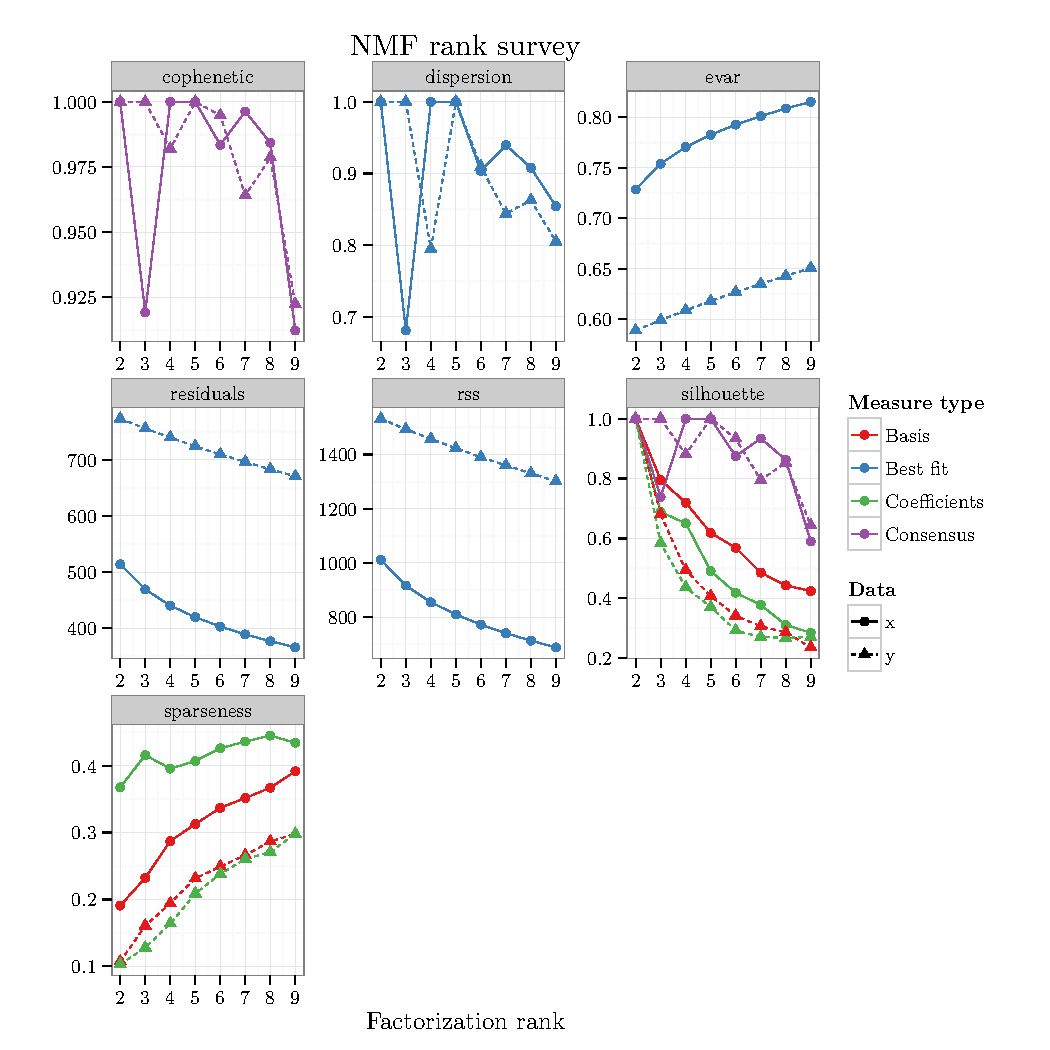
\includegraphics[width=\maxwidth]{figure/nmf-rank-plots-1} 

}


\begin{kframe}\begin{alltt}
\hlkwd{plot}\hlstd{(nmf.rankrange[}\hlopt{-}\hlnum{1}\hlstd{],} \hlopt{-}\hlstd{temp.orig_resids.delta,}
        \hlkwc{type} \hlstd{=} \hlstr{"o"}\hlstd{,} \hlkwc{col} \hlstd{=} \hlstr{"black"}\hlstd{,} \hlkwc{pch} \hlstd{=} \hlnum{21}\hlstd{,} \hlkwc{ylim} \hlstd{=} \hlkwd{range}\hlstd{(}\hlopt{-}\hlkwd{c}\hlstd{(temp.orig_resids.delta, temp.perm_resids.delta.mean)),}
        \hlkwc{xlab} \hlstd{=} \hlstr{"Factorization Rank Added"}\hlstd{,} \hlkwc{ylab} \hlstd{=} \hlstr{"Improvement in Total Residual Error"}\hlstd{)}
\hlkwd{lines}\hlstd{(nmf.rankrange[}\hlopt{-}\hlnum{1}\hlstd{],} \hlopt{-}\hlstd{temp.perm_resids.delta.mean,} \hlkwc{col} \hlstd{=} \hlstr{"red"}\hlstd{,} \hlkwc{type} \hlstd{=} \hlstr{"o"}\hlstd{,} \hlkwc{pch} \hlstd{=} \hlnum{21}\hlstd{,} \hlkwc{lwd} \hlstd{=} \hlnum{1}\hlstd{)}
\hlkwa{for} \hlstd{(i} \hlkwa{in} \hlnum{1}\hlopt{:}\hlkwd{ncol}\hlstd{(temp.perm_resids))}
\hlstd{\{}
        \hlkwd{lines}\hlstd{(nmf.rankrange[}\hlopt{-}\hlnum{1}\hlstd{],} \hlopt{-}\hlstd{temp.perm_resids.delta[,i],} \hlkwc{type} \hlstd{=} \hlstr{"o"}\hlstd{,} \hlkwc{col} \hlstd{=} \hlkwd{rgb}\hlstd{(}\hlnum{1}\hlstd{,} \hlnum{0}\hlstd{,} \hlnum{0}\hlstd{,} \hlnum{0.25}\hlstd{))}
\hlstd{\}}
\hlkwd{lines}\hlstd{(nmf.rankrange[}\hlopt{-}\hlnum{1}\hlstd{],} \hlopt{-}\hlstd{temp.perm_resids.delta.threshold,} \hlkwc{col} \hlstd{=} \hlstr{"red"}\hlstd{,} \hlkwc{lty} \hlstd{=} \hlstr{"dotted"}\hlstd{)}
\hlkwa{if} \hlstd{(nmf.rank.wasauto} \hlopt{==} \hlnum{TRUE}\hlstd{)}
\hlstd{\{}
        \hlstd{temp.col} \hlkwb{=} \hlstr{"green"}
\hlstd{\}} \hlkwa{else} \hlstd{\{}
        \hlstd{temp.col} \hlkwb{=} \hlstr{"blue"}
\hlstd{\}}
\hlkwd{abline}\hlstd{(}\hlkwc{v} \hlstd{= nmf.rank,} \hlkwc{col} \hlstd{= temp.col,} \hlkwc{lwd} \hlstd{=} \hlnum{2}\hlstd{)}
\hlkwd{legend}\hlstd{(}\hlstr{"topright"}\hlstd{,} \hlkwc{legend} \hlstd{=} \hlkwd{c}\hlstd{(}\hlstr{"Original data"}\hlstd{,} \hlstr{"Permuted data"}\hlstd{,} \hlkwd{sprintf}\hlstd{(}\hlstr{"Selected rank (%s)"}\hlstd{,} \hlkwd{ifelse}\hlstd{(nmf.rank.wasauto} \hlopt{==} \hlnum{TRUE}\hlstd{,} \hlstr{"auto"}\hlstd{,} \hlstr{"fixed"}\hlstd{))),} \hlkwc{col} \hlstd{=} \hlkwd{c}\hlstd{(}\hlstr{"black"}\hlstd{,} \hlstr{"red"}\hlstd{, temp.col),}  \hlkwc{lty} \hlstd{=} \hlstr{"solid"}\hlstd{,} \hlkwc{pch} \hlstd{=} \hlnum{21}\hlstd{,} \hlkwc{inset} \hlstd{=} \hlnum{0.05}\hlstd{)}
\end{alltt}
\end{kframe}

{\centering 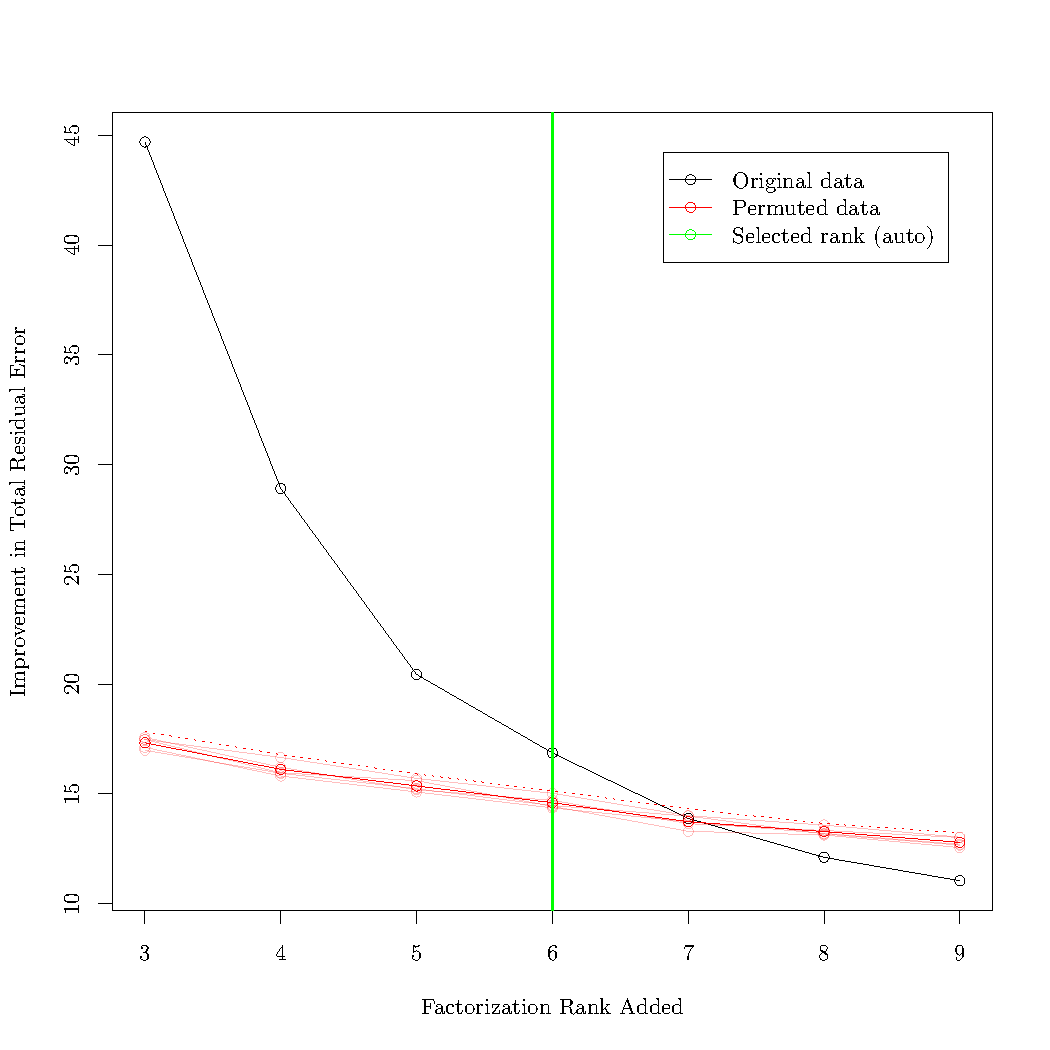
\includegraphics[width=\maxwidth]{figure/nmf-rank-plots-2} 

}



\end{knitrout}

\subsection{Fit}
\begin{knitrout}
\definecolor{shadecolor}{rgb}{0.969, 0.969, 0.969}\color{fgcolor}\begin{kframe}
\begin{alltt}
\hlkwd{consensusmap}\hlstd{(nmf.final)}
\end{alltt}
\end{kframe}

{\centering 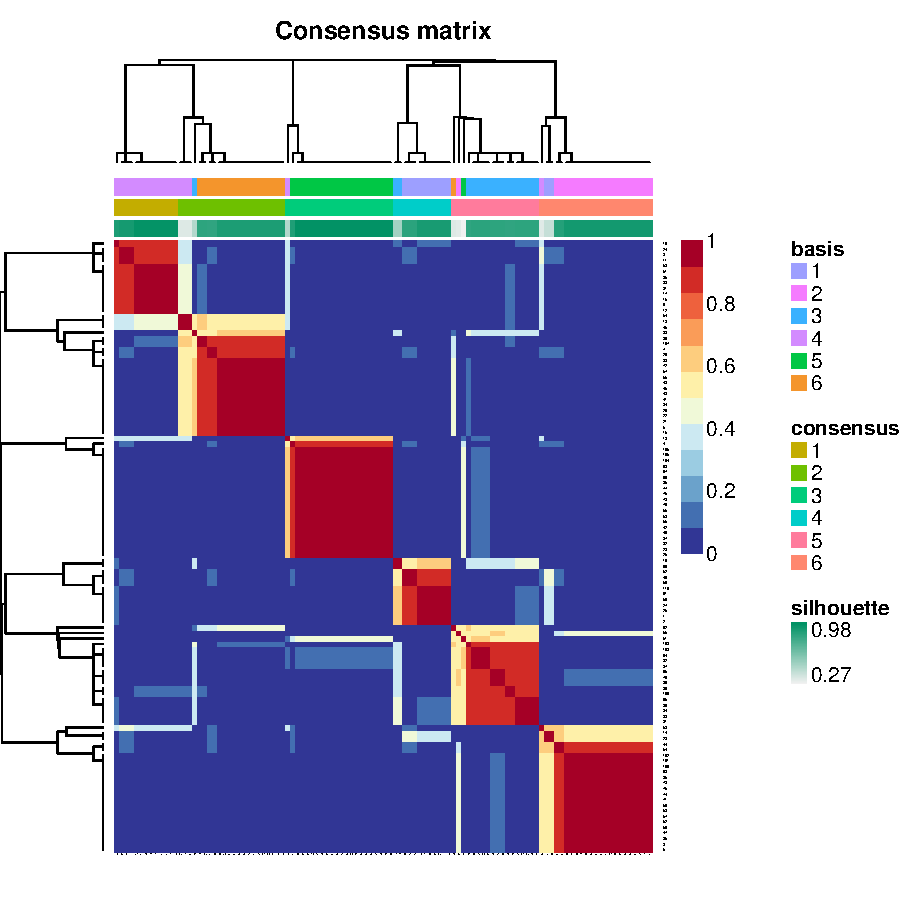
\includegraphics[width=\maxwidth]{figure/nmf-plots-1} 

}


\begin{kframe}\begin{alltt}
\hlkwd{basismap}\hlstd{(nmf.final)}
\end{alltt}
\end{kframe}

{\centering 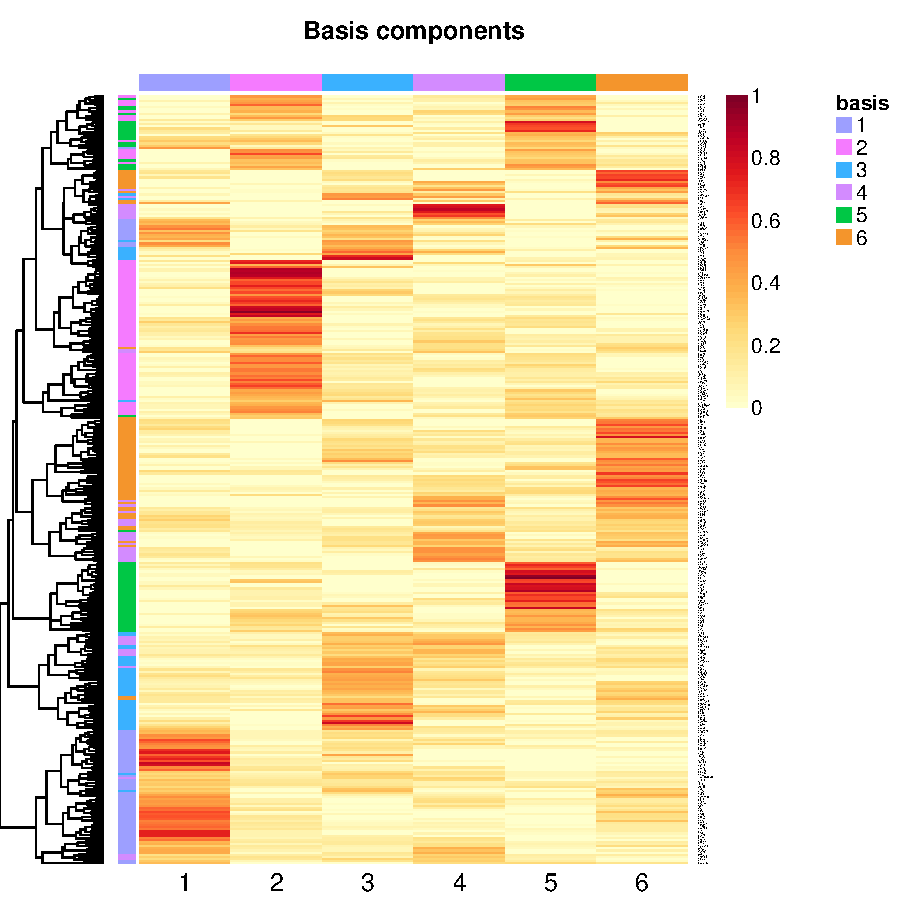
\includegraphics[width=\maxwidth]{figure/nmf-plots-2} 

}


\begin{kframe}\begin{alltt}
\hlkwd{coefmap}\hlstd{(nmf.final)}
\end{alltt}
\end{kframe}

{\centering 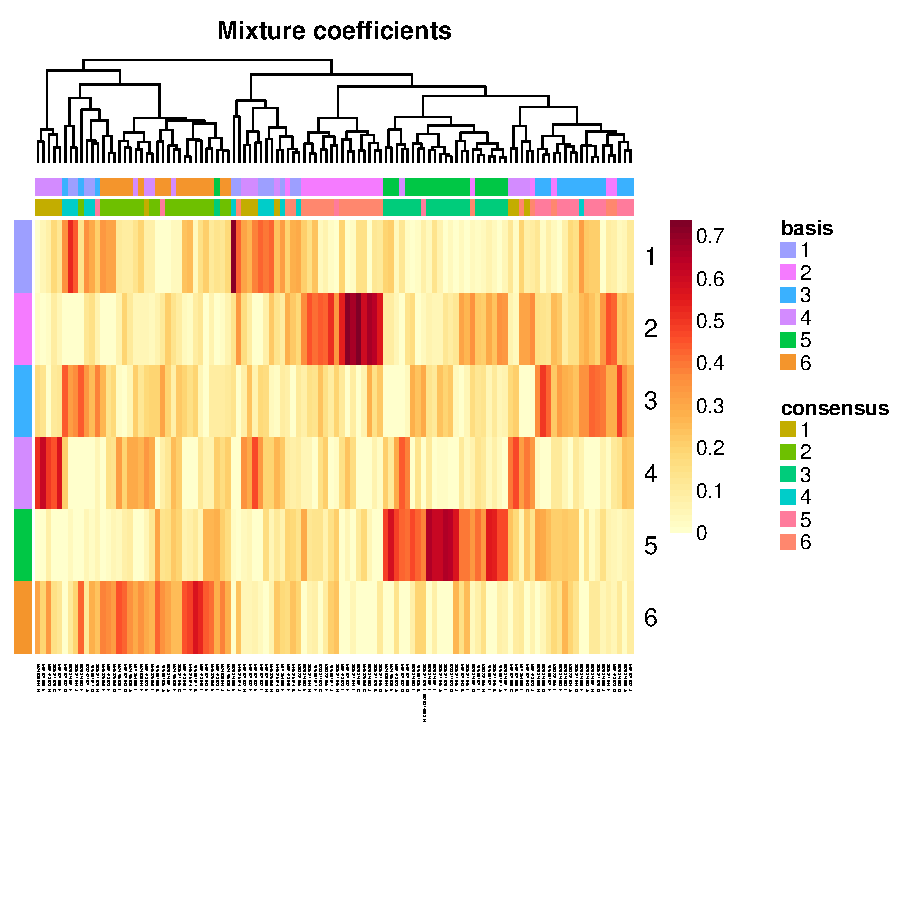
\includegraphics[width=\maxwidth]{figure/nmf-plots-3} 

}



\end{knitrout}


%%%%%%%%%%%%%%%%%%%%%%%%%%%%%%%%%%%%%%%%%%%%%%%%%%%%%%%%%%%%%%%%%%%%%%
% SIGNATURE ESTIMATION
%%%%%%%%%%%%%%%%%%%%%%%%%%%%%%%%%%%%%%%%%%%%%%%%%%%%%%%%%%%%%%%%%%%%%%
\begin{knitrout}
\definecolor{shadecolor}{rgb}{0.969, 0.969, 0.969}\color{fgcolor}\begin{kframe}
\begin{alltt}
\hlstd{coefs.diag_dsd} \hlkwb{=} \hlkwd{apply}\hlstd{(xlin.diag_dsd.sel,} \hlnum{2}\hlstd{,} \hlkwa{function}\hlstd{(}\hlkwc{xcol}\hlstd{)} \hlkwd{nnls}\hlstd{(}\hlkwd{basis}\hlstd{(nmf.final), xcol)}\hlopt{$}\hlstd{x)}
\hlstd{coefs.diag_rec} \hlkwb{=} \hlkwd{apply}\hlstd{(xlin.diag_rec.sel,} \hlnum{2}\hlstd{,} \hlkwa{function}\hlstd{(}\hlkwc{xcol}\hlstd{)} \hlkwd{nnls}\hlstd{(}\hlkwd{basis}\hlstd{(nmf.final), xcol)}\hlopt{$}\hlstd{x)}
\hlstd{coefs.recr_dsd} \hlkwb{=} \hlkwd{apply}\hlstd{(xlin.recr_dsd.sel,} \hlnum{2}\hlstd{,} \hlkwa{function}\hlstd{(}\hlkwc{xcol}\hlstd{)} \hlkwd{nnls}\hlstd{(}\hlkwd{basis}\hlstd{(nmf.final), xcol)}\hlopt{$}\hlstd{x)}
\hlstd{coefs.pdac_au} \hlkwb{=} \hlkwd{apply}\hlstd{(xlin.pdac_au.sel,} \hlnum{2}\hlstd{,} \hlkwa{function}\hlstd{(}\hlkwc{xcol}\hlstd{)} \hlkwd{nnls}\hlstd{(}\hlkwd{basis}\hlstd{(nmf.final), xcol)}\hlopt{$}\hlstd{x)}
\hlstd{axis_coefs.diag_dsd} \hlkwb{=} \hlkwd{as.matrix}\hlstd{(}\hlkwd{cbind}\hlstd{(}\hlkwc{axis1} \hlstd{= coefs.diag_dsd[}\hlnum{1}\hlstd{,]} \hlopt{-} \hlstd{coefs.diag_dsd[}\hlnum{5}\hlstd{,],} \hlkwc{axis2} \hlstd{= coefs.diag_dsd[}\hlnum{6}\hlstd{,]} \hlopt{-} \hlstd{coefs.diag_dsd[}\hlnum{2}\hlstd{,]))}
\end{alltt}
\end{kframe}
\end{knitrout}


%%%%%%%%%%%%%%%%%%%%%%%%%%%%%%%%%%%%%%%%%%%%%%%%%%%%%%%%%%%%%%%%%%%%%%
% METAGENE BASIS SAVING, PARSE APPROXIMATION
%%%%%%%%%%%%%%%%%%%%%%%%%%%%%%%%%%%%%%%%%%%%%%%%%%%%%%%%%%%%%%%%%%%%%%


\begin{knitrout}
\definecolor{shadecolor}{rgb}{0.969, 0.969, 0.969}\color{fgcolor}\begin{kframe}
\begin{alltt}
\hlkwd{library}\hlstd{(MASS)}
\hlstd{W_plus} \hlkwb{=} \hlkwd{ginv}\hlstd{(}\hlkwd{basis}\hlstd{(nmf.final))}

\hlstd{A1} \hlkwb{=} \hlstd{W_plus[}\hlnum{1}\hlstd{,]} \hlopt{-} \hlstd{W_plus[}\hlnum{5}\hlstd{,]}
\hlstd{A2} \hlkwb{=} \hlstd{W_plus[}\hlnum{6}\hlstd{,]} \hlopt{-} \hlstd{W_plus[}\hlnum{2}\hlstd{,]}
\hlstd{PARSE_approx} \hlkwb{=} \hlkwd{matrix}\hlstd{(}\hlnum{1.354}\hlopt{*}\hlstd{A1} \hlopt{+} \hlnum{1.548}\hlopt{*}\hlstd{A2,} \hlkwc{ncol} \hlstd{=} \hlnum{1}\hlstd{)}

\hlkwd{rownames}\hlstd{(PARSE_approx)} \hlkwb{=} \hlkwd{rownames}\hlstd{(}\hlkwd{basis}\hlstd{(nmf.final))}

\hlstd{PARSE_approx_scores} \hlkwb{=} \hlkwd{t}\hlstd{(xlin.diag_dsd.sel)} \hlopt \hlstd{PARSE_approx}
\hlstd{PARSE_exact_scores} \hlkwb{=} \hlnum{1.354}\hlopt{*}\hlstd{(coefs.diag_dsd[}\hlnum{1}\hlstd{,]} \hlopt{-} \hlstd{coefs.diag_dsd[}\hlnum{5}\hlstd{,])} \hlopt{+} \hlnum{1.548}\hlopt{*}\hlstd{(coefs.diag_dsd[}\hlnum{6}\hlstd{,]} \hlopt{-} \hlstd{coefs.diag_dsd[}\hlnum{2}\hlstd{,])}

\hlkwd{plot}\hlstd{(PARSE_exact_scores, PARSE_approx_scores,} \hlkwc{xlab} \hlstd{=} \hlstr{"Exact PARSE score"}\hlstd{,} \hlkwc{ylab} \hlstd{=} \hlstr{"Approximate PARSE score"}\hlstd{)}
\hlkwd{abline}\hlstd{(}\hlnum{0}\hlstd{,} \hlnum{1}\hlstd{,} \hlkwc{col} \hlstd{=} \hlkwd{rgb}\hlstd{(}\hlnum{0}\hlstd{,} \hlnum{0}\hlstd{,} \hlnum{0}\hlstd{,} \hlnum{0.25}\hlstd{))}
\end{alltt}
\end{kframe}

{\centering 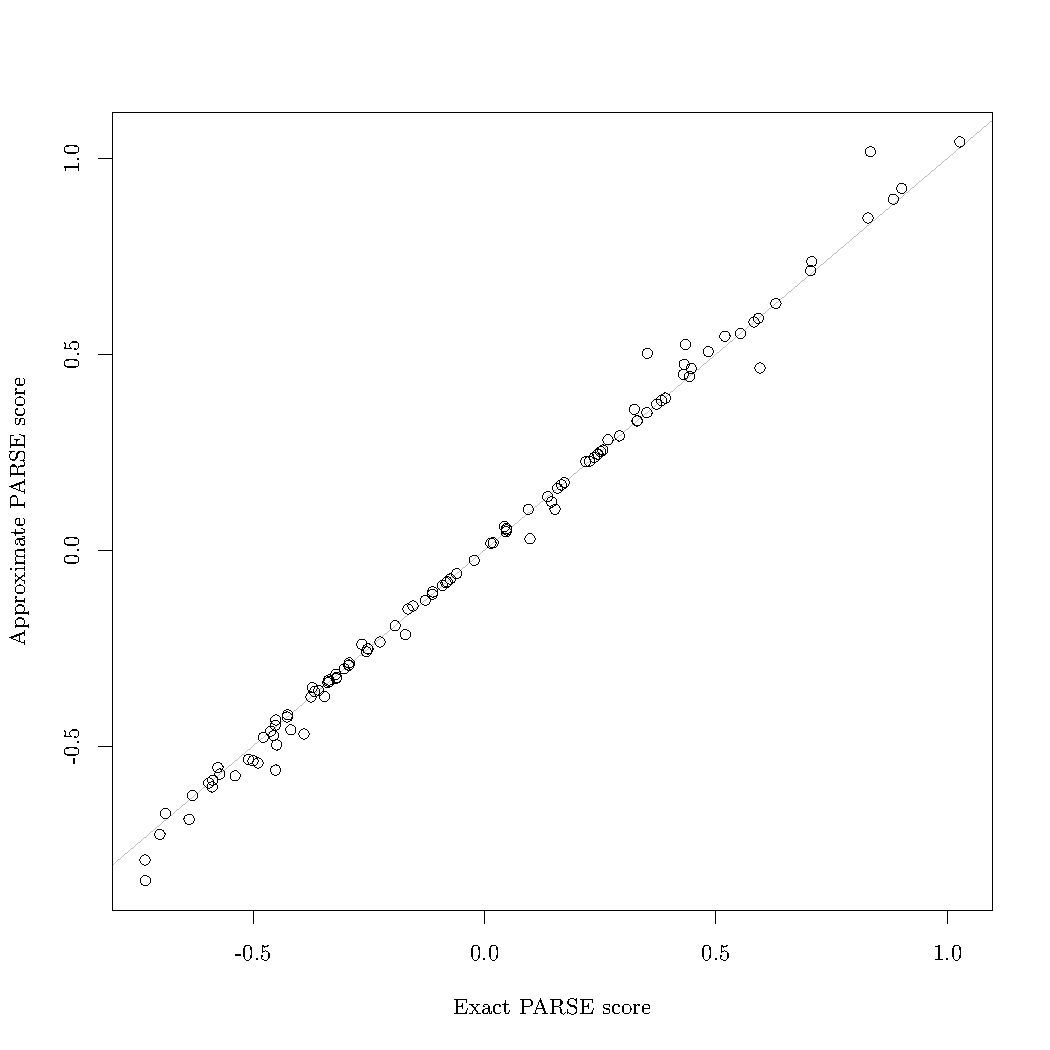
\includegraphics[width=\maxwidth]{figure/approx-calc-1} 

}



\end{knitrout}





%%%%%%%%%%%%%%%%%%%%%%%%%%%%%%%%%%%%%%%%%%%%%%%%%%%%%%%%%%%%%%%%%%%%%%
% METAGENE PAIRING, AXES
%%%%%%%%%%%%%%%%%%%%%%%%%%%%%%%%%%%%%%%%%%%%%%%%%%%%%%%%%%%%%%%%%%%%%%

\begin{knitrout}
\definecolor{shadecolor}{rgb}{0.969, 0.969, 0.969}\color{fgcolor}\begin{kframe}
\begin{alltt}
\hlstd{temp.pred.pairs} \hlkwb{=} \hlkwd{t}\hlstd{(}\hlkwd{rbind}\hlstd{(coefs.pdac_au, metapcna.scores[}\hlkwd{colnames}\hlstd{(coefs.pdac_au)]))}
\hlkwd{colnames}\hlstd{(temp.pred.pairs)} \hlkwb{=} \hlkwd{paste}\hlstd{(}\hlstr{"mg"}\hlstd{,} \hlnum{1}\hlopt{:}\hlkwd{ncol}\hlstd{(temp.pred.pairs),} \hlkwc{sep} \hlstd{=} \hlstr{"."}\hlstd{)}
\hlkwd{colnames}\hlstd{(temp.pred.pairs)[}\hlkwd{ncol}\hlstd{(temp.pred.pairs)]} \hlkwb{=} \hlstr{"PCNA"}
\hlstd{temp.pred.pairs} \hlkwb{=} \hlkwd{cbind}\hlstd{(temp.pred.pairs,} \hlkwc{qpure} \hlstd{= samps.pdac_au}\hlopt{$}\hlstd{purity_qpure,} \hlkwc{pkyrs} \hlstd{= cpvs.pdac_au}\hlopt{$}\hlstd{History.Smoking.PackYears)}
\hlkwd{pairs}\hlstd{(temp.pred.pairs,} \hlkwc{pch} \hlstd{=} \hlnum{16}\hlstd{,} \hlkwc{cex} \hlstd{=} \hlnum{1}\hlstd{,} \hlkwc{col} \hlstd{=} \hlkwd{ifelse}\hlstd{(}\hlkwd{rownames}\hlstd{(temp.pred.pairs)} \hlopt \hlkwd{colnames}\hlstd{(xlin.diag_dsd.sel),} \hlkwd{rgb}\hlstd{(}\hlnum{0}\hlstd{,} \hlnum{0}\hlstd{,} \hlnum{0}\hlstd{,} \hlnum{0.5}\hlstd{),} \hlkwd{rgb}\hlstd{(}\hlnum{1}\hlstd{,} \hlnum{0}\hlstd{,} \hlnum{1}\hlstd{,} \hlnum{0.5}\hlstd{)))}
\end{alltt}
\end{kframe}

{\centering 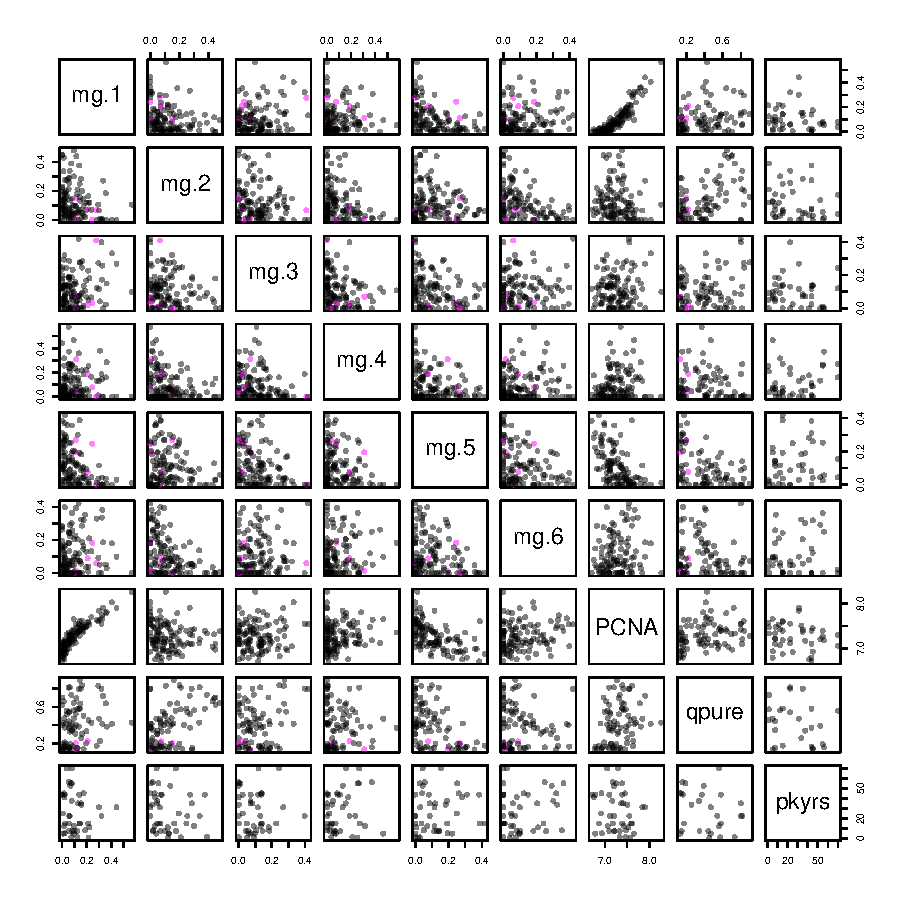
\includegraphics[width=\maxwidth]{figure/metagene-pairs-1} 

}


\begin{kframe}\begin{alltt}
\hlstd{temp.pred.pairs.rescaled} \hlkwb{=} \hlkwd{t}\hlstd{((}\hlkwd{t}\hlstd{(temp.pred.pairs)} \hlopt{-} \hlkwd{apply}\hlstd{(temp.pred.pairs,} \hlnum{2}\hlstd{, min,} \hlkwc{na.rm} \hlstd{=} \hlnum{TRUE}\hlstd{))} \hlopt{/} \hlstd{(}\hlkwd{apply}\hlstd{(temp.pred.pairs,} \hlnum{2}\hlstd{,} \hlkwa{function}\hlstd{(}\hlkwc{x}\hlstd{)} \hlkwd{diff}\hlstd{(}\hlkwd{range}\hlstd{(x,} \hlkwc{na.rm} \hlstd{=} \hlnum{TRUE}\hlstd{)))))}
\hlkwd{heatmap.2}\hlstd{(temp.pred.pairs.rescaled,} \hlkwc{trace} \hlstd{=} \hlstr{"none"}\hlstd{,} \hlkwc{scale} \hlstd{=} \hlstr{"none"}\hlstd{,} \hlkwc{col} \hlstd{=} \hlkwd{brewer.pal}\hlstd{(}\hlnum{9}\hlstd{,} \hlstr{"GnBu"}\hlstd{))}
\end{alltt}
\end{kframe}

{\centering 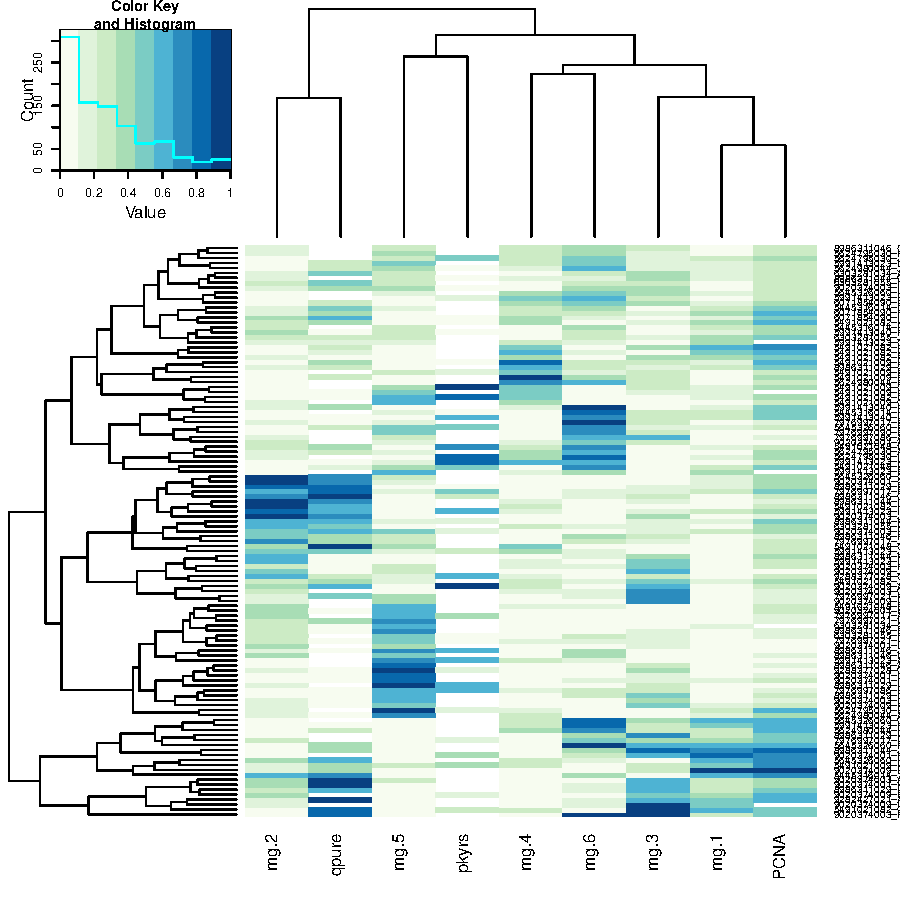
\includegraphics[width=\maxwidth]{figure/metagene-pairs-2} 

}


\begin{kframe}\begin{alltt}
\hlkwd{heatmap.2}\hlstd{(temp.pred.pairs.rescaled[}\hlkwd{apply}\hlstd{(}\hlopt{!}\hlkwd{is.na}\hlstd{(temp.pred.pairs.rescaled),} \hlnum{1}\hlstd{, all),],} \hlkwc{trace} \hlstd{=} \hlstr{"none"}\hlstd{,} \hlkwc{scale} \hlstd{=} \hlstr{"none"}\hlstd{,} \hlkwc{col} \hlstd{=} \hlkwd{brewer.pal}\hlstd{(}\hlnum{9}\hlstd{,} \hlstr{"GnBu"}\hlstd{))}
\end{alltt}
\end{kframe}

{\centering 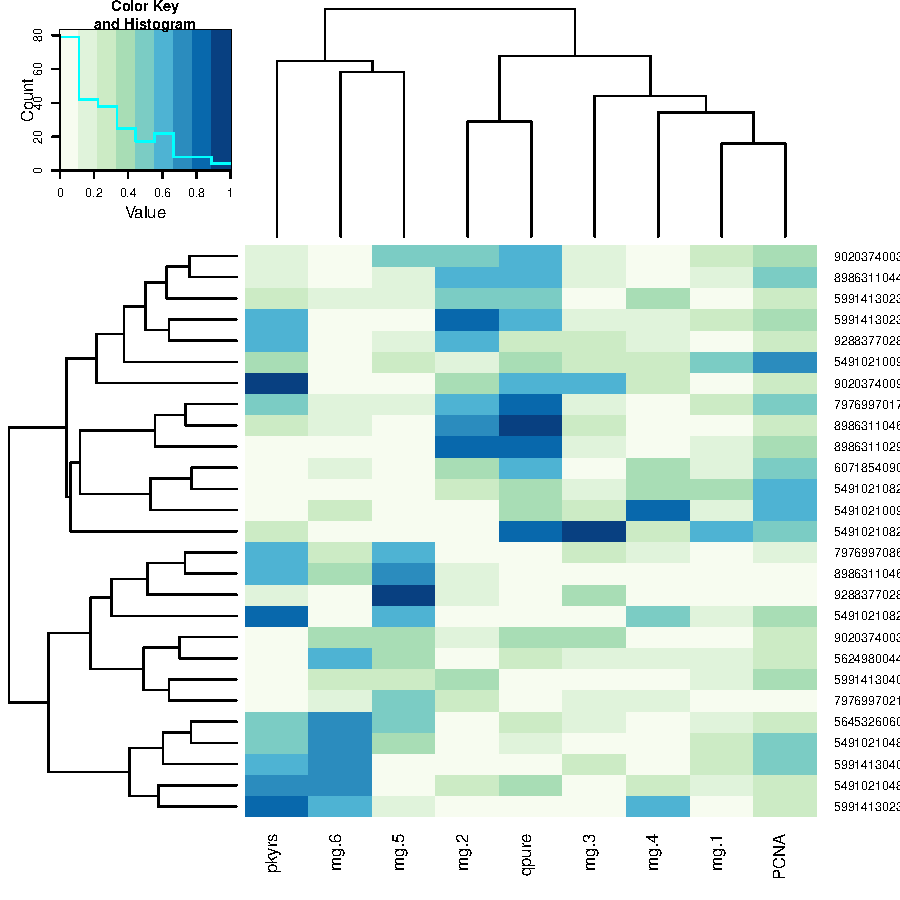
\includegraphics[width=\maxwidth]{figure/metagene-pairs-3} 

}


\begin{kframe}\begin{alltt}
\hlstd{temp.pred.pairs.rescaled2} \hlkwb{=} \hlstd{temp.pred.pairs.rescaled[,}\hlkwd{colnames}\hlstd{(temp.pred.pairs.rescaled)} \hlopt{!=} \hlstr{"pkyrs"}\hlstd{]}
\hlkwd{heatmap.2}\hlstd{(temp.pred.pairs.rescaled2,} \hlkwc{trace} \hlstd{=} \hlstr{"none"}\hlstd{,} \hlkwc{scale} \hlstd{=} \hlstr{"none"}\hlstd{,} \hlkwc{col} \hlstd{=} \hlkwd{brewer.pal}\hlstd{(}\hlnum{9}\hlstd{,} \hlstr{"GnBu"}\hlstd{))}
\end{alltt}
\end{kframe}

{\centering 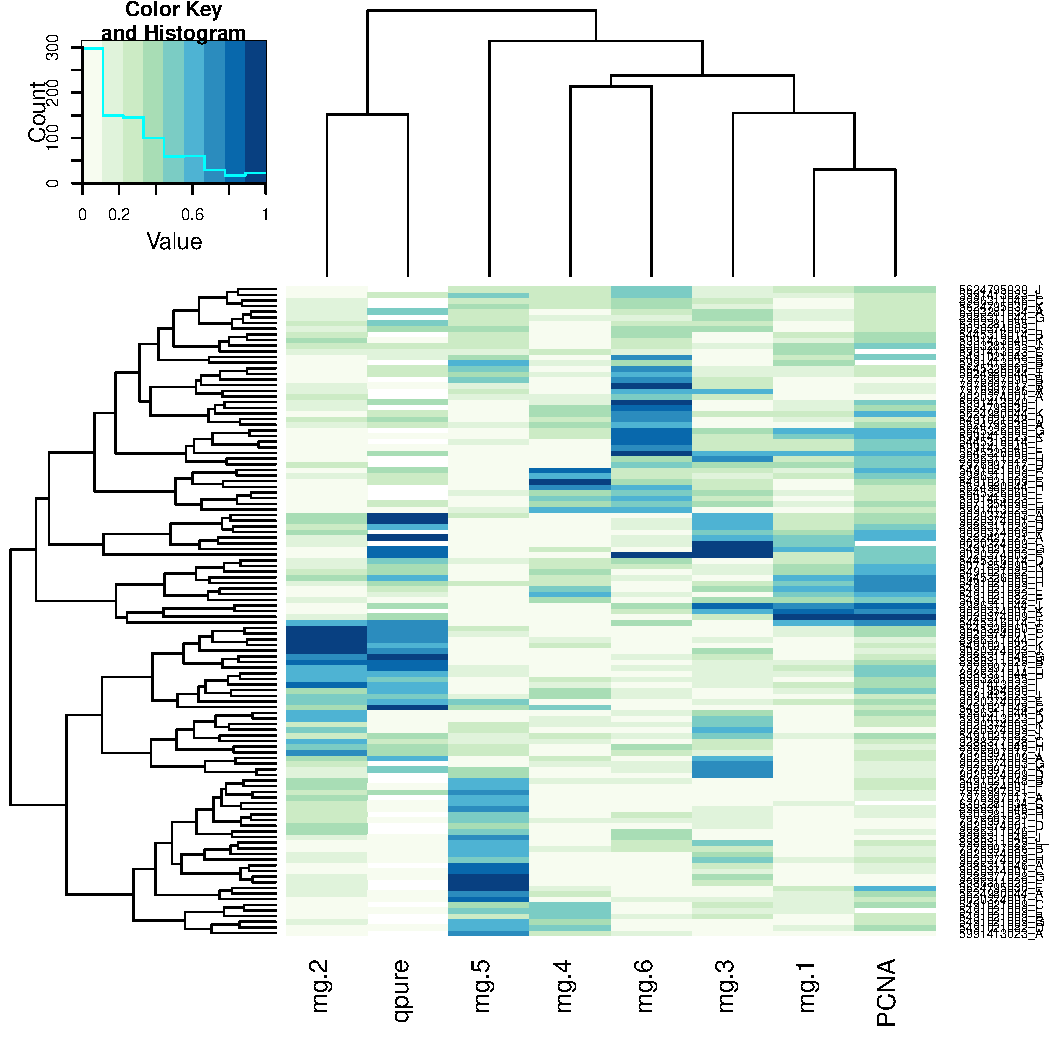
\includegraphics[width=\maxwidth]{figure/metagene-pairs-4} 

}


\begin{kframe}\begin{alltt}
\hlkwd{heatmap.2}\hlstd{(temp.pred.pairs.rescaled2[}\hlkwd{apply}\hlstd{(}\hlopt{!}\hlkwd{is.na}\hlstd{(temp.pred.pairs.rescaled2),} \hlnum{1}\hlstd{, all),],} \hlkwc{trace} \hlstd{=} \hlstr{"none"}\hlstd{,} \hlkwc{scale} \hlstd{=} \hlstr{"none"}\hlstd{,} \hlkwc{col} \hlstd{=} \hlkwd{brewer.pal}\hlstd{(}\hlnum{9}\hlstd{,} \hlstr{"GnBu"}\hlstd{))}
\end{alltt}
\end{kframe}

{\centering 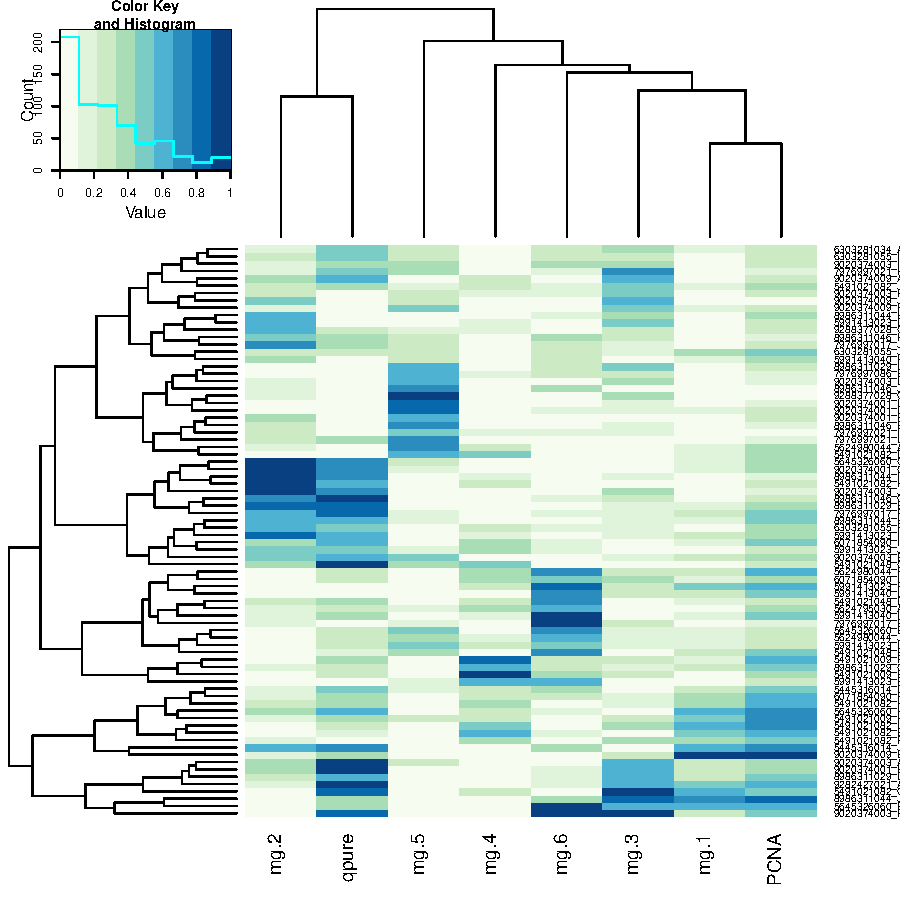
\includegraphics[width=\maxwidth]{figure/metagene-pairs-5} 

}


\begin{kframe}\begin{alltt}
\hlstd{temp.cors} \hlkwb{=} \hlkwd{apply}\hlstd{(temp.pred.pairs[,}\hlkwd{colnames}\hlstd{(temp.pred.pairs)} \hlopt{!=} \hlstr{"pkyrs"}\hlstd{],} \hlnum{2}\hlstd{,} \hlkwa{function}\hlstd{(}\hlkwc{x}\hlstd{)} \hlkwd{apply}\hlstd{(temp.pred.pairs[,}\hlkwd{colnames}\hlstd{(temp.pred.pairs)} \hlopt{!=} \hlstr{"pkyrs"}\hlstd{],} \hlnum{2}\hlstd{,} \hlkwa{function}\hlstd{(}\hlkwc{y}\hlstd{) \{ sel} \hlkwb{=} \hlopt{!}\hlstd{(}\hlkwd{is.na}\hlstd{(x)} \hlopt{|} \hlkwd{is.na}\hlstd{(y));} \hlkwd{cor}\hlstd{(x[sel], y[sel],} \hlkwc{method} \hlstd{=} \hlstr{"kendall"}\hlstd{) \} ))}
\hlcom{#diag(temp.cors) = NA}
\hlkwd{heatmap.2}\hlstd{(temp.cors,} \hlkwc{trace} \hlstd{=} \hlstr{"none"}\hlstd{,} \hlkwc{Rowv} \hlstd{=} \hlnum{FALSE}\hlstd{,} \hlkwc{Colv} \hlstd{=} \hlnum{FALSE}\hlstd{,} \hlkwc{col} \hlstd{=} \hlkwd{brewer.pal}\hlstd{(}\hlnum{11}\hlstd{,} \hlstr{"PiYG"}\hlstd{),} \hlkwc{dendrogram} \hlstd{=} \hlstr{"none"}\hlstd{,} \hlkwc{scale} \hlstd{=} \hlstr{"none"}\hlstd{)}
\end{alltt}
\end{kframe}

{\centering 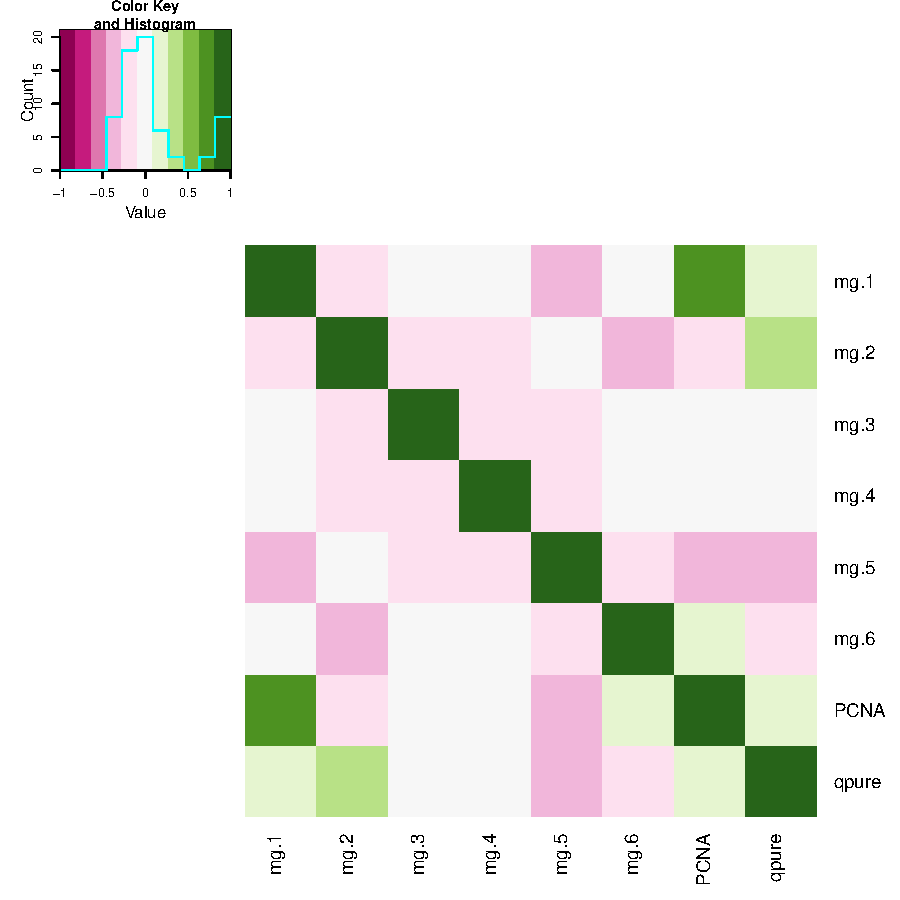
\includegraphics[width=\maxwidth]{figure/metagene-pairs-6} 

}


\begin{kframe}\begin{alltt}
\hlkwd{plot}\hlstd{(temp.pred.pairs[,}\hlstr{"mg.1"}\hlstd{]} \hlopt{~} \hlstd{temp.pred.pairs[,}\hlstr{"PCNA"}\hlstd{],} \hlkwc{col} \hlstd{=} \hlkwd{ifelse}\hlstd{(}\hlkwd{rownames}\hlstd{(temp.pred.pairs)} \hlopt \hlkwd{colnames}\hlstd{(xlin.diag_dsd.sel),} \hlkwd{rgb}\hlstd{(}\hlnum{0}\hlstd{,} \hlnum{0}\hlstd{,} \hlnum{0}\hlstd{,} \hlnum{1}\hlstd{),} \hlkwd{rgb}\hlstd{(}\hlnum{0}\hlstd{,} \hlnum{0}\hlstd{,} \hlnum{0}\hlstd{,} \hlnum{0}\hlstd{)),} \hlkwc{xlab} \hlstd{=} \hlstr{"Meta-PCNA Score"}\hlstd{,} \hlkwc{ylab} \hlstd{=} \hlstr{"MG1 Coefficient"}\hlstd{)}
\end{alltt}
\end{kframe}

{\centering 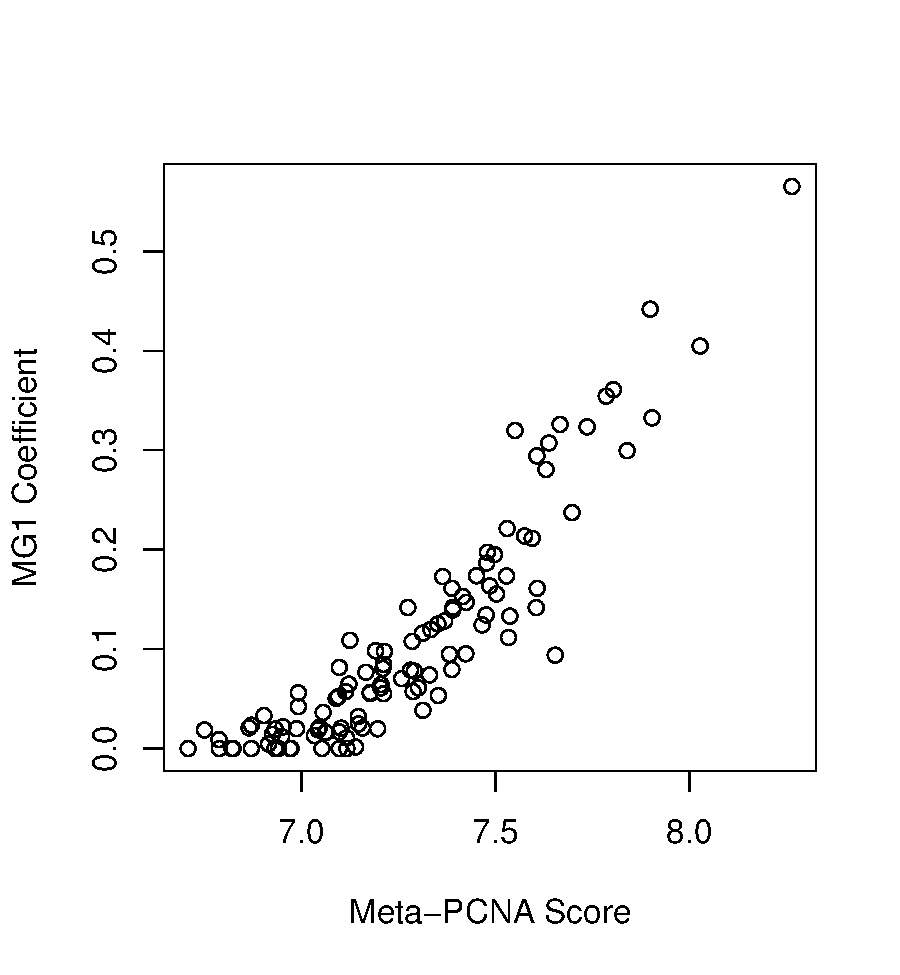
\includegraphics[width=\maxwidth]{figure/metagene-pairs-7} 

}


\begin{kframe}\begin{alltt}
\hlkwd{plot}\hlstd{(temp.pred.pairs[,}\hlstr{"mg.5"}\hlstd{], temp.pred.pairs[,}\hlstr{"mg.1"}\hlstd{],} \hlkwc{xlab} \hlstd{=} \hlstr{"MG5 Coefficient (protective)"}\hlstd{,} \hlkwc{ylab} \hlstd{=} \hlstr{"MG1 Coefficient (hazardous)"}\hlstd{)}
\end{alltt}
\end{kframe}

{\centering 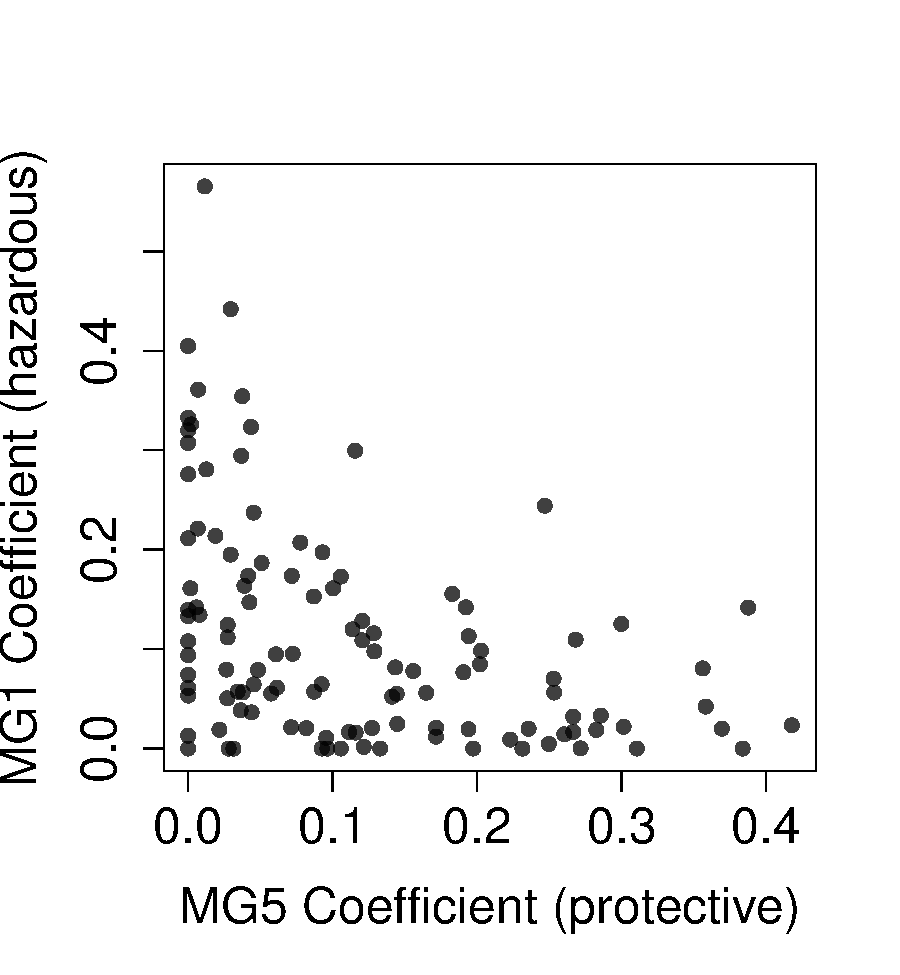
\includegraphics[width=\maxwidth]{figure/metagene-pairs-8} 

}


\begin{kframe}\begin{alltt}
\hlkwd{plot}\hlstd{(temp.pred.pairs[,}\hlstr{"mg.2"}\hlstd{], temp.pred.pairs[,}\hlstr{"mg.6"}\hlstd{],} \hlkwc{xlab} \hlstd{=} \hlstr{"MG2 Coefficient (protective)"}\hlstd{,} \hlkwc{ylab} \hlstd{=} \hlstr{"MG6 Coefficient"}\hlstd{)}
\end{alltt}
\end{kframe}

{\centering 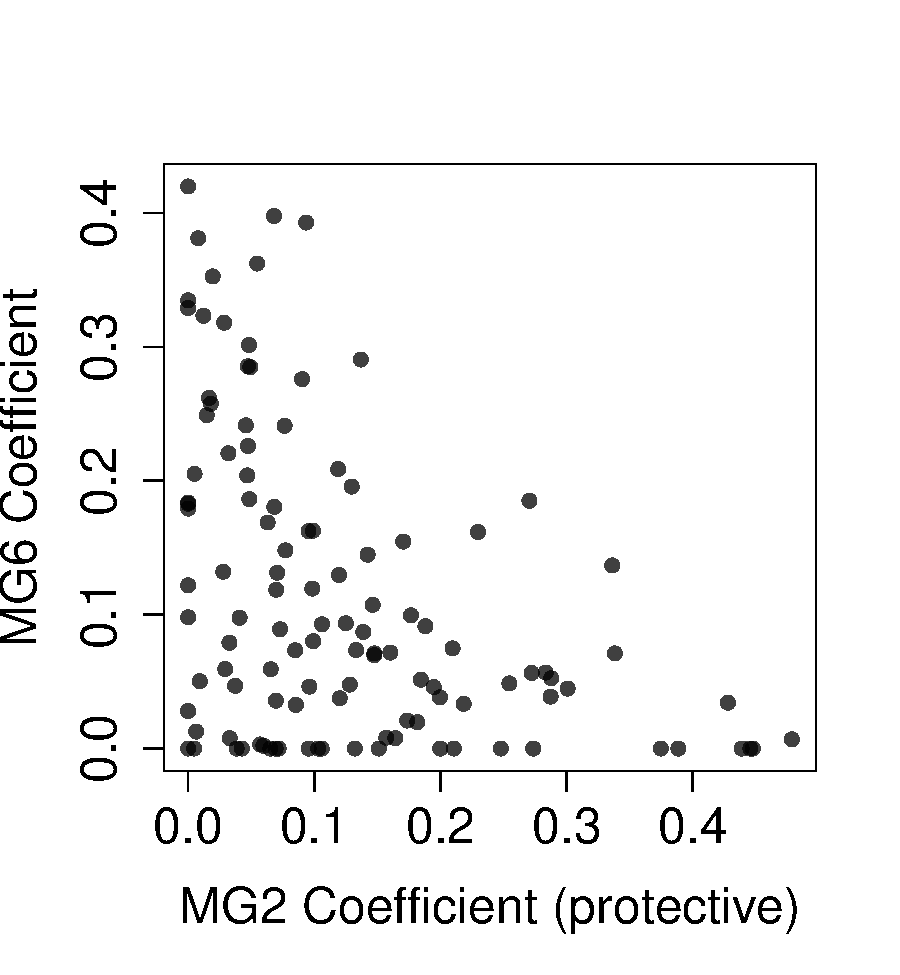
\includegraphics[width=\maxwidth]{figure/metagene-pairs-9} 

}


\begin{kframe}\begin{alltt}
\hlcom{#scatter.smooth(temp.pred.pairs[,"mg.5"], temp.pred.pairs[,"mg.1"], xlab = "MG5 Coefficient (protective)", ylab = "MG1 Coefficient (hazardous)", span = 1/4, lpars = list(lwd = 2, col = rgb(0, 0, 0, 0.5)))}
\hlcom{#scatter.smooth(temp.pred.pairs[,"mg.2"], temp.pred.pairs[,"mg.6"], xlab = "MG2 Coefficient (protective)", ylab = "MG6 Coefficient", span = 1/4, lpars = list(lwd = 2, col = rgb(0, 0, 1, 0.5)))}
\hlcom{#smoothScatter(temp.pred.pairs[,"mg.5"], temp.pred.pairs[,"mg.1"], xlab = "MG5 Coefficient (protective)", ylab = "MG1 Coefficient (hazardous)")}
\hlcom{#smoothScatter(temp.pred.pairs[,"mg.2"], temp.pred.pairs[,"mg.6"], xlab = "MG2 Coefficient (protective)", ylab = "MG6 Coefficient")}

\hlstd{temp.coefs.pdcor} \hlkwb{=} \hlkwd{apply}\hlstd{(coefs.diag_dsd,} \hlnum{1}\hlstd{,} \hlkwa{function}\hlstd{(}\hlkwc{x1}\hlstd{)} \hlkwd{apply}\hlstd{(coefs.diag_dsd,} \hlnum{1}\hlstd{,} \hlkwa{function}\hlstd{(}\hlkwc{x2}\hlstd{)} \hlkwd{dcov.test}\hlstd{(x1, x2,} \hlkwc{R} \hlstd{=} \hlnum{9999}\hlstd{)}\hlopt{$}\hlstd{p.value))}
\hlstd{temp.coefs.pfisher} \hlkwb{=} \hlkwd{apply}\hlstd{(coefs.diag_dsd,} \hlnum{1}\hlstd{,} \hlkwa{function}\hlstd{(}\hlkwc{x1}\hlstd{)} \hlkwd{apply}\hlstd{(coefs.diag_dsd,} \hlnum{1}\hlstd{,} \hlkwa{function}\hlstd{(}\hlkwc{x2}\hlstd{)} \hlkwd{fisher.test}\hlstd{(x1} \hlopt{>} \hlkwd{median}\hlstd{(x1), x2} \hlopt{>} \hlkwd{median}\hlstd{(x2))}\hlopt{$}\hlstd{p.value))}
\hlkwd{diag}\hlstd{(temp.coefs.pdcor)} \hlkwb{=} \hlnum{NA}
\hlstd{temp.coefs.pdcor[}\hlkwd{lower.tri}\hlstd{(temp.coefs.pdcor)]} \hlkwb{=} \hlnum{NA}
\hlkwd{diag}\hlstd{(temp.coefs.pfisher)} \hlkwb{=} \hlnum{NA}
\hlstd{temp.coefs.pfisher[}\hlkwd{lower.tri}\hlstd{(temp.coefs.pfisher)]} \hlkwb{=} \hlnum{NA}
\hlstd{temp.coefs.pdcor.holm} \hlkwb{=} \hlkwd{matrix}\hlstd{(}\hlkwd{p.adjust}\hlstd{(temp.coefs.pdcor,} \hlstr{"holm"}\hlstd{),} \hlkwc{nrow} \hlstd{=} \hlkwd{nrow}\hlstd{(temp.coefs.pdcor))}
\hlstd{temp.coefs.pfisher.holm} \hlkwb{=} \hlkwd{matrix}\hlstd{(}\hlkwd{p.adjust}\hlstd{(temp.coefs.pfisher,} \hlstr{"holm"}\hlstd{),} \hlkwc{nrow} \hlstd{=} \hlkwd{nrow}\hlstd{(temp.coefs.pfisher))}
\hlstd{temp.coefs.pdcor.holm}
\end{alltt}
\begin{verbatim}
##      [,1]   [,2]   [,3]   [,4]   [,5]   [,6]
## [1,]   NA 0.1848 0.4540 1.0000 0.0015 1.0000
## [2,]   NA     NA 0.3276 0.0299 0.1576 0.0015
## [3,]   NA     NA     NA 0.0385 0.0312 1.0000
## [4,]   NA     NA     NA     NA 0.0558 1.0000
## [5,]   NA     NA     NA     NA     NA 0.0385
## [6,]   NA     NA     NA     NA     NA     NA
\end{verbatim}
\begin{alltt}
\hlstd{temp.coefs.pfisher.holm}
\end{alltt}
\begin{verbatim}
##      [,1] [,2]   [,3] [,4]    [,5]    [,6]
## [1,]   NA    1 1.0000    1 0.03203 1.00000
## [2,]   NA   NA 0.7286    1 1.00000 0.03203
## [3,]   NA   NA     NA    1 1.00000 1.00000
## [4,]   NA   NA     NA   NA 0.72858 1.00000
## [5,]   NA   NA     NA   NA      NA 1.00000
## [6,]   NA   NA     NA   NA      NA      NA
\end{verbatim}
\begin{alltt}
\hlkwd{dcov.test}\hlstd{(coefs.diag_dsd[}\hlnum{5}\hlstd{,], coefs.diag_dsd[}\hlnum{1}\hlstd{,],} \hlkwc{R} \hlstd{=} \hlnum{19999}\hlstd{)}
\end{alltt}
\begin{verbatim}
## 
## 	dCov test of independence
## 
## data:  index 1, replicates 19999
## nV^2 = 0.1291, p-value = 5e-05
## sample estimates:
##    dCov 
## 0.03426
\end{verbatim}
\begin{alltt}
\hlkwd{dcov.test}\hlstd{(coefs.diag_dsd[}\hlnum{2}\hlstd{,], coefs.diag_dsd[}\hlnum{6}\hlstd{,],} \hlkwc{R} \hlstd{=} \hlnum{19999}\hlstd{)}
\end{alltt}
\begin{verbatim}
## 
## 	dCov test of independence
## 
## data:  index 1, replicates 19999
## nV^2 = 0.1396, p-value = 5e-05
## sample estimates:
##    dCov 
## 0.03562
\end{verbatim}
\begin{alltt}
\hlkwd{cor.test}\hlstd{(coefs.diag_dsd[}\hlnum{5}\hlstd{,], coefs.diag_dsd[}\hlnum{1}\hlstd{,],} \hlkwc{method} \hlstd{=} \hlstr{"kendall"}\hlstd{)}
\end{alltt}
\begin{verbatim}
## 
## 	Kendall's rank correlation tau
## 
## data:  coefs.diag_dsd[5, ] and coefs.diag_dsd[1, ]
## z = -4.97, p-value = 6.694e-07
## alternative hypothesis: true tau is not equal to 0
## sample estimates:
##     tau 
## -0.3243
\end{verbatim}
\begin{alltt}
\hlkwd{cor.test}\hlstd{(coefs.diag_dsd[}\hlnum{2}\hlstd{,], coefs.diag_dsd[}\hlnum{6}\hlstd{,],} \hlkwc{method} \hlstd{=} \hlstr{"kendall"}\hlstd{)}
\end{alltt}
\begin{verbatim}
## 
## 	Kendall's rank correlation tau
## 
## data:  coefs.diag_dsd[2, ] and coefs.diag_dsd[6, ]
## z = -4.931, p-value = 8.195e-07
## alternative hypothesis: true tau is not equal to 0
## sample estimates:
##     tau 
## -0.3236
\end{verbatim}
\begin{alltt}
\hlstd{temp.axis1} \hlkwb{=} \hlstd{coefs.diag_dsd[}\hlnum{1}\hlstd{,]} \hlopt{-} \hlstd{coefs.diag_dsd[}\hlnum{5}\hlstd{,]}
\hlstd{temp.axis2} \hlkwb{=} \hlstd{coefs.diag_dsd[}\hlnum{6}\hlstd{,]} \hlopt{-} \hlstd{coefs.diag_dsd[}\hlnum{2}\hlstd{,]}
\hlkwd{dcov.test}\hlstd{(temp.axis1, temp.axis2,} \hlkwc{R} \hlstd{=} \hlnum{19999}\hlstd{)}
\end{alltt}
\begin{verbatim}
## 
## 	dCov test of independence
## 
## data:  index 1, replicates 19999
## nV^2 = 0.1074, p-value = 0.02035
## sample estimates:
##    dCov 
## 0.03124
\end{verbatim}
\begin{alltt}
\hlkwd{cor.test}\hlstd{(temp.axis1, temp.axis2,} \hlkwc{method} \hlstd{=} \hlstr{"kendall"}\hlstd{)}
\end{alltt}
\begin{verbatim}
## 
## 	Kendall's rank correlation tau
## 
## data:  temp.axis1 and temp.axis2
## z = 1.253, p-value = 0.2103
## alternative hypothesis: true tau is not equal to 0
## sample estimates:
##    tau 
## 0.0809
\end{verbatim}
\begin{alltt}
\hlkwd{plot}\hlstd{(temp.axis2} \hlopt{~} \hlstd{temp.axis1,} \hlkwc{xlab} \hlstd{=} \hlstr{"Axis 1 activity"}\hlstd{,} \hlkwc{ylab} \hlstd{=} \hlstr{"Axis 2 activity"}\hlstd{)}
\end{alltt}
\end{kframe}

{\centering 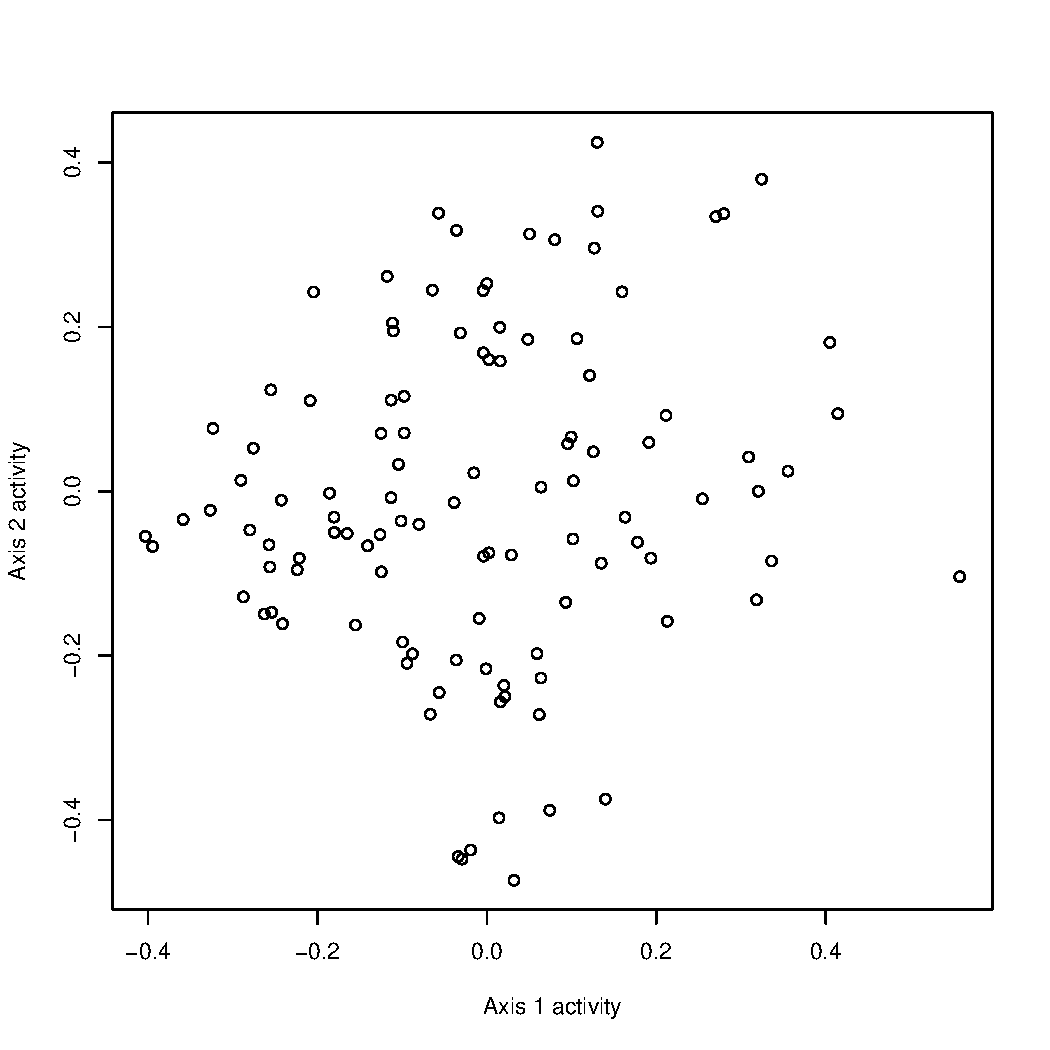
\includegraphics[width=\maxwidth]{figure/metagene-pairs-10} 

}


\begin{kframe}\begin{alltt}
\hlkwd{coxph}\hlstd{(y.diag_dsd} \hlopt{~} \hlstd{temp.axis1} \hlopt{*} \hlstd{temp.axis2)}
\end{alltt}
\begin{verbatim}
## Call:
## coxph(formula = y.diag_dsd ~ temp.axis1 * temp.axis2)
## 
## 
##                       coef exp(coef) se(coef)    z       p
## temp.axis1            3.19      24.2    0.676 4.72 2.4e-06
## temp.axis2            2.89      18.0    0.657 4.40 1.1e-05
## temp.axis1:temp.axis2 5.03     153.1    4.189 1.20 2.3e-01
## 
## Likelihood ratio test=48  on 3 df, p=2.12e-10  n= 110, number of events= 70
\end{verbatim}
\begin{alltt}
\hlstd{temp} \hlkwb{=} \hlkwd{cv.glmnet}\hlstd{(}\hlkwd{cbind}\hlstd{(temp.axis1, temp.axis2, temp.axis1}\hlopt{*}\hlstd{temp.axis2), y.diag_dsd,} \hlkwc{family} \hlstd{=} \hlstr{"cox"}\hlstd{,} \hlkwc{nfolds} \hlstd{=} \hlnum{10}\hlstd{)}
\hlkwd{plot}\hlstd{(temp)}
\end{alltt}
\end{kframe}

{\centering 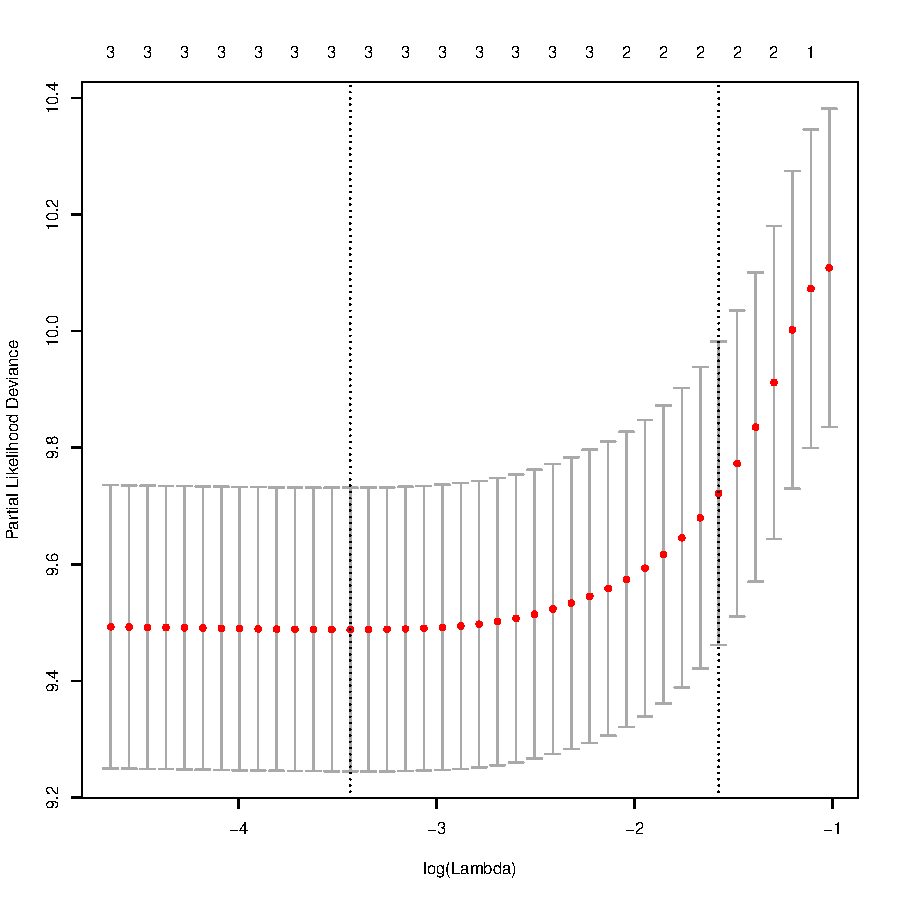
\includegraphics[width=\maxwidth]{figure/metagene-pairs-11} 

}


\begin{kframe}\begin{alltt}
\hlkwd{plot}\hlstd{(temp}\hlopt{$}\hlstd{glmnet.fit,} \hlkwc{label} \hlstd{=} \hlnum{TRUE}\hlstd{)}
\hlkwd{abline}\hlstd{(}\hlkwc{v} \hlstd{=} \hlkwd{sum}\hlstd{(}\hlkwd{abs}\hlstd{(}\hlkwd{coef}\hlstd{(temp}\hlopt{$}\hlstd{glmnet.fit,} \hlkwc{s} \hlstd{= temp}\hlopt{$}\hlstd{lambda.1se))))}
\hlkwd{abline}\hlstd{(}\hlkwc{v} \hlstd{=} \hlkwd{sum}\hlstd{(}\hlkwd{abs}\hlstd{(}\hlkwd{coef}\hlstd{(temp}\hlopt{$}\hlstd{glmnet.fit,} \hlkwc{s} \hlstd{= temp}\hlopt{$}\hlstd{lambda.min))))}
\end{alltt}
\end{kframe}

{\centering 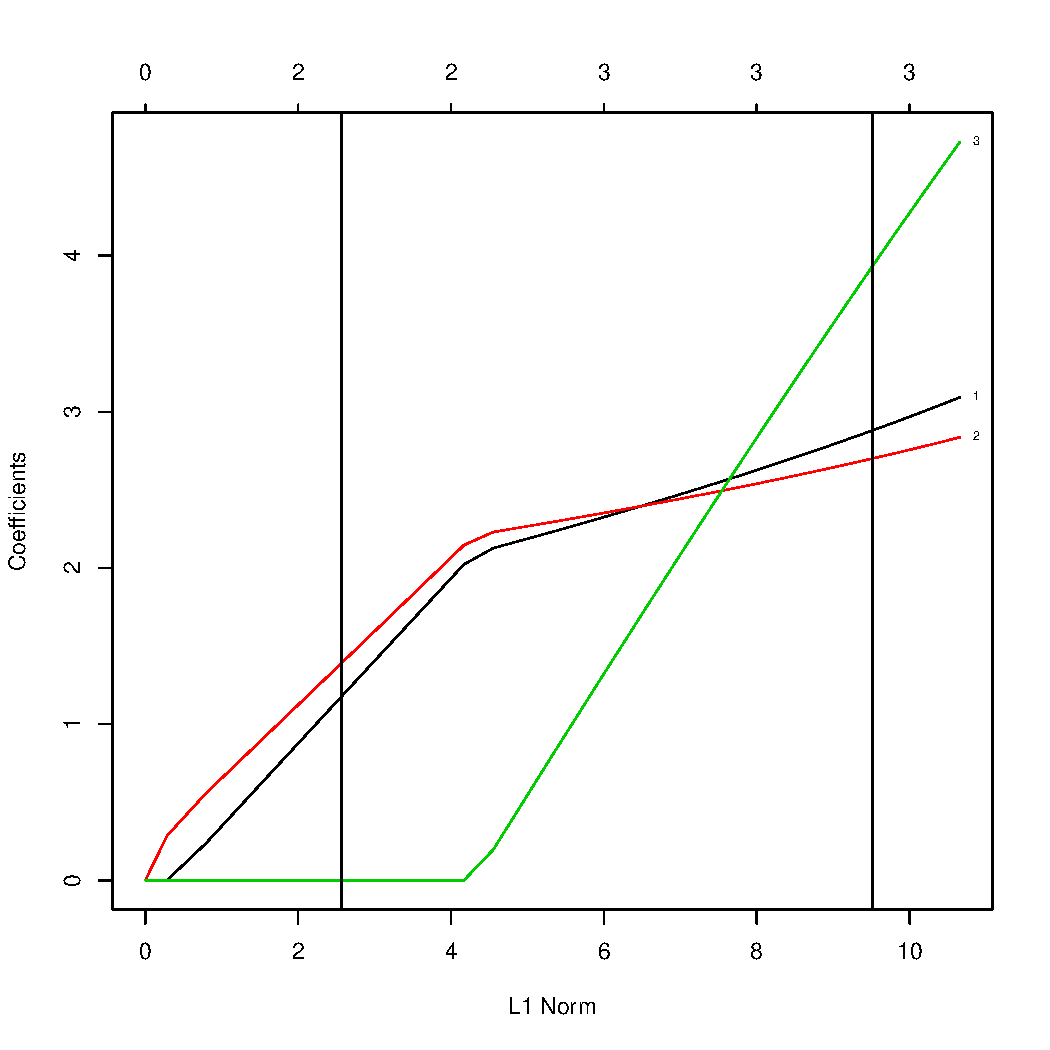
\includegraphics[width=\maxwidth]{figure/metagene-pairs-12} 

}


\begin{kframe}\begin{alltt}
\hlkwd{coef}\hlstd{(temp}\hlopt{$}\hlstd{glmnet.fit,} \hlkwc{s} \hlstd{= temp}\hlopt{$}\hlstd{lambda.1se)}
\end{alltt}
\begin{verbatim}
## 3 x 1 sparse Matrix of class "dgCMatrix"
##                 1
## temp.axis1 0.7582
## temp.axis2 1.0185
##            .
\end{verbatim}
\end{kframe}
\end{knitrout}


%%%%%%%%%%%%%%%%%%%%%%%%%%%%%%%%%%%%%%%%%%%%%%%%%%%%%%%%%%%%%%%%%%%%%%
% SIGNATURE PROGNOSTIC PERFORMANCE: TRAINING SET, ALONE
%%%%%%%%%%%%%%%%%%%%%%%%%%%%%%%%%%%%%%%%%%%%%%%%%%%%%%%%%%%%%%%%%%%%%%
\subsection{LASSO on training set}
\begin{knitrout}
\definecolor{shadecolor}{rgb}{0.969, 0.969, 0.969}\color{fgcolor}\begin{kframe}
\begin{alltt}
\hlstd{glmnet.fit.cv.diag_dsd} \hlkwb{=} \hlkwd{cv.glmnet}\hlstd{(}\hlkwd{t}\hlstd{(coefs.diag_dsd), y.diag_dsd,} \hlkwc{family} \hlstd{=} \hlstr{"cox"}\hlstd{,} \hlkwc{nfolds} \hlstd{=} \hlnum{10}\hlstd{)}
\hlstd{glmnet.fit.cv.diag_rec} \hlkwb{=} \hlkwd{cv.glmnet}\hlstd{(}\hlkwd{t}\hlstd{(coefs.diag_rec), y.diag_rec,} \hlkwc{family} \hlstd{=} \hlstr{"cox"}\hlstd{,} \hlkwc{nfolds} \hlstd{=} \hlnum{10}\hlstd{)}
\hlstd{glmnet.fit.cv.recr_dsd} \hlkwb{=} \hlkwd{cv.glmnet}\hlstd{(}\hlkwd{t}\hlstd{(coefs.recr_dsd), y.recr_dsd,} \hlkwc{family} \hlstd{=} \hlstr{"cox"}\hlstd{,} \hlkwc{nfolds} \hlstd{=} \hlnum{10}\hlstd{)}
\end{alltt}
\end{kframe}
\end{knitrout}

\begin{knitrout}
\definecolor{shadecolor}{rgb}{0.969, 0.969, 0.969}\color{fgcolor}\begin{kframe}
\begin{alltt}
\hlkwd{plot}\hlstd{(glmnet.fit.cv.diag_dsd)}
\end{alltt}
\end{kframe}

{\centering 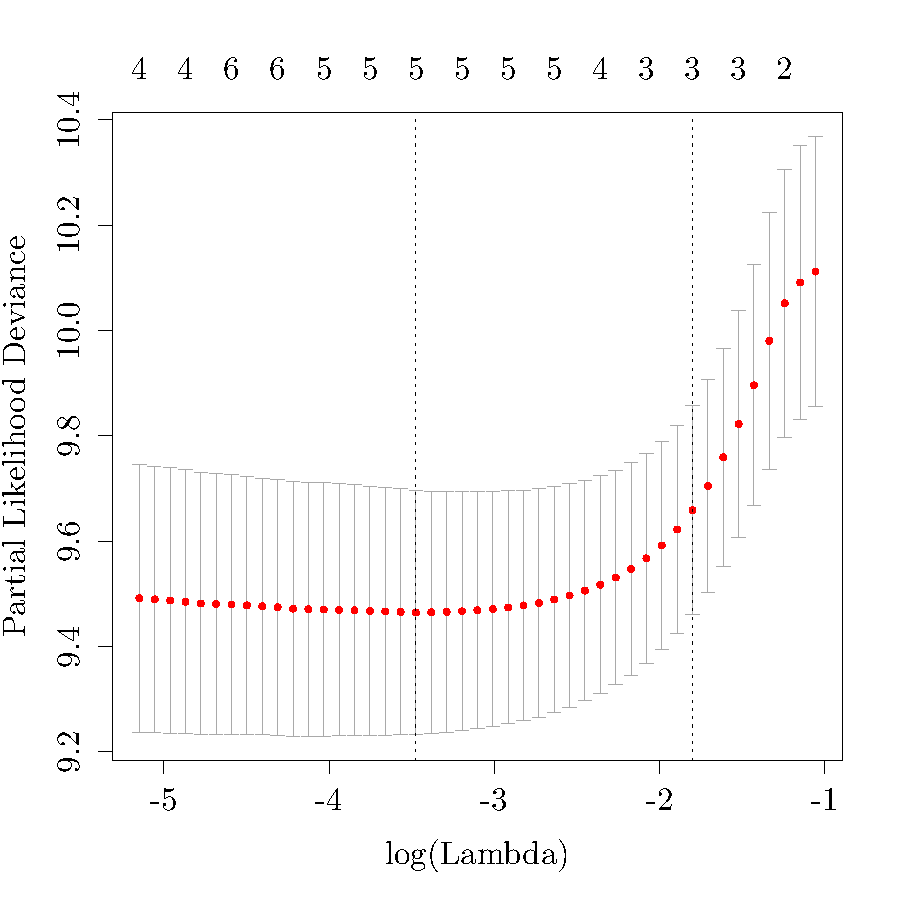
\includegraphics[width=\maxwidth]{figure/nmf-metagene-glmnet-plots-1} 

}


\begin{kframe}\begin{alltt}
\hlkwd{plot}\hlstd{(glmnet.fit.cv.diag_dsd}\hlopt{$}\hlstd{glmnet.fit,} \hlkwc{label} \hlstd{=} \hlnum{TRUE}\hlstd{)}
\hlkwd{abline}\hlstd{(}\hlkwc{v} \hlstd{=} \hlkwd{sum}\hlstd{(}\hlkwd{abs}\hlstd{(}\hlkwd{coef}\hlstd{(glmnet.fit.cv.diag_dsd}\hlopt{$}\hlstd{glmnet.fit,} \hlkwc{s} \hlstd{= glmnet.fit.cv.diag_dsd}\hlopt{$}\hlstd{lambda.1se))))}
\end{alltt}
\end{kframe}

{\centering 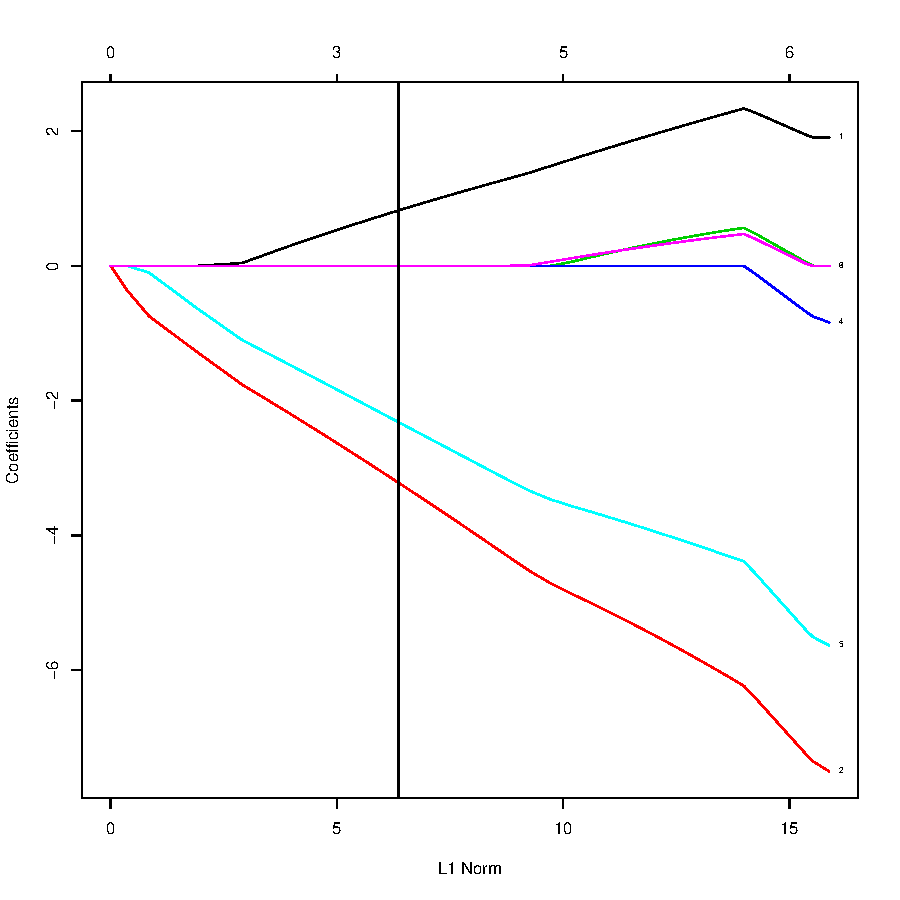
\includegraphics[width=\maxwidth]{figure/nmf-metagene-glmnet-plots-2} 

}


\begin{kframe}\begin{alltt}
\hlcom{#abline(v = sum(abs(coef(glmnet.fit.cv.diag_dsd$glmnet.fit, s = glmnet.fit.cv.diag_dsd$lambda.min))))}
\hlkwd{coef}\hlstd{(glmnet.fit.cv.diag_dsd}\hlopt{$}\hlstd{glmnet.fit,} \hlkwc{s} \hlstd{= glmnet.fit.cv.diag_dsd}\hlopt{$}\hlstd{lambda.1se)}
\end{alltt}
\begin{verbatim}
## 6 x 1 sparse Matrix of class "dgCMatrix"
##          1
## V1  0.9616
## V2 -3.5221
## V3  .     
## V4  .     
## V5 -2.5631
## V6  .
\end{verbatim}
\begin{alltt}
\hlkwd{plot}\hlstd{(glmnet.fit.cv.diag_rec)}
\end{alltt}
\end{kframe}

{\centering 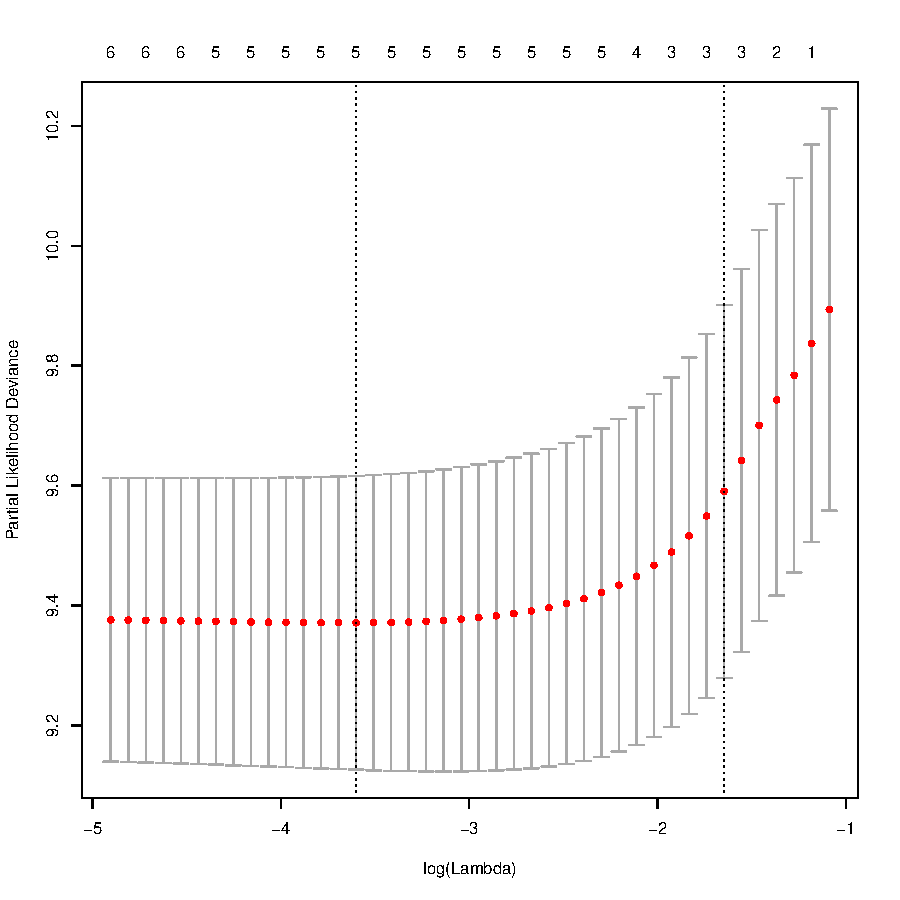
\includegraphics[width=\maxwidth]{figure/nmf-metagene-glmnet-plots-3} 

}


\begin{kframe}\begin{alltt}
\hlkwd{plot}\hlstd{(glmnet.fit.cv.diag_rec}\hlopt{$}\hlstd{glmnet.fit,} \hlkwc{label} \hlstd{=} \hlnum{TRUE}\hlstd{)}
\hlkwd{abline}\hlstd{(}\hlkwc{v} \hlstd{=} \hlkwd{sum}\hlstd{(}\hlkwd{abs}\hlstd{(}\hlkwd{coef}\hlstd{(glmnet.fit.cv.diag_rec}\hlopt{$}\hlstd{glmnet.fit,} \hlkwc{s} \hlstd{= glmnet.fit.cv.diag_rec}\hlopt{$}\hlstd{lambda.1se))))}
\end{alltt}
\end{kframe}

{\centering 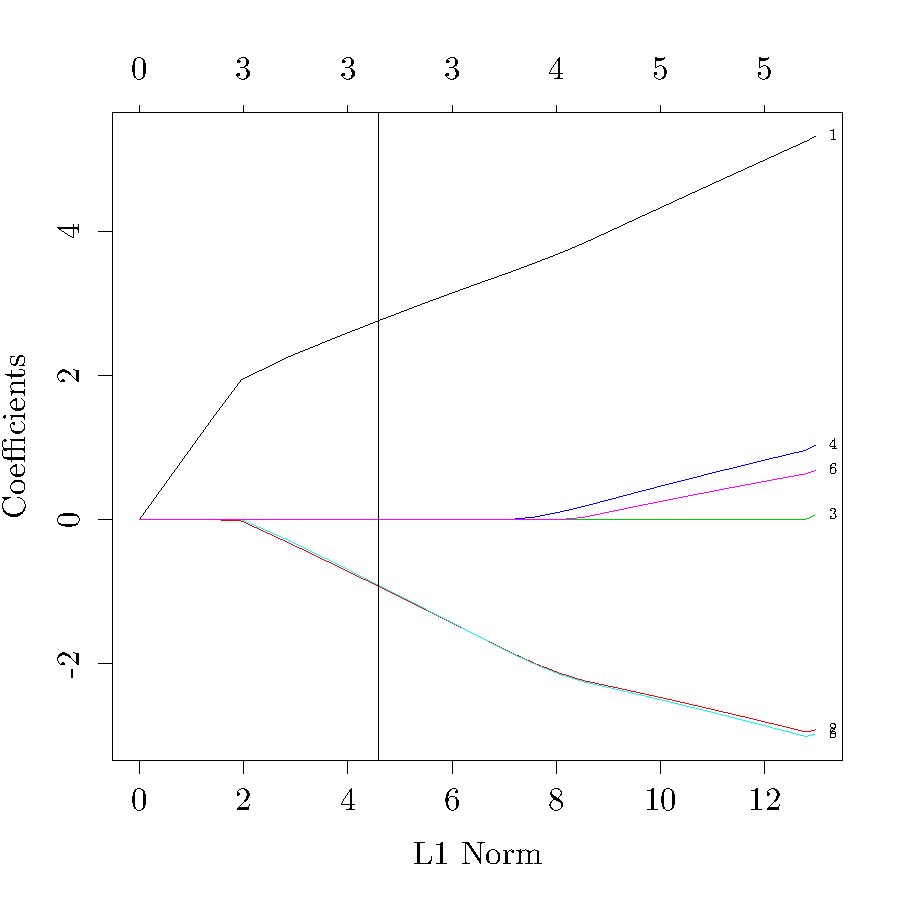
\includegraphics[width=\maxwidth]{figure/nmf-metagene-glmnet-plots-4} 

}


\begin{kframe}\begin{alltt}
\hlcom{#abline(v = sum(abs(coef(glmnet.fit.cv.diag_rec$glmnet.fit, s = glmnet.fit.cv.diag_rec$lambda.min))))}
\hlkwd{coef}\hlstd{(glmnet.fit.cv.diag_rec}\hlopt{$}\hlstd{glmnet.fit,} \hlkwc{s} \hlstd{= glmnet.fit.cv.diag_rec}\hlopt{$}\hlstd{lambda.1se)}
\end{alltt}
\begin{verbatim}
## 6 x 1 sparse Matrix of class "dgCMatrix"
##          1
## V1  2.2667
## V2 -0.3332
## V3  .     
## V4  .     
## V5 -0.2974
## V6  .
\end{verbatim}
\begin{alltt}
\hlkwd{plot}\hlstd{(glmnet.fit.cv.recr_dsd)}
\end{alltt}
\end{kframe}

{\centering 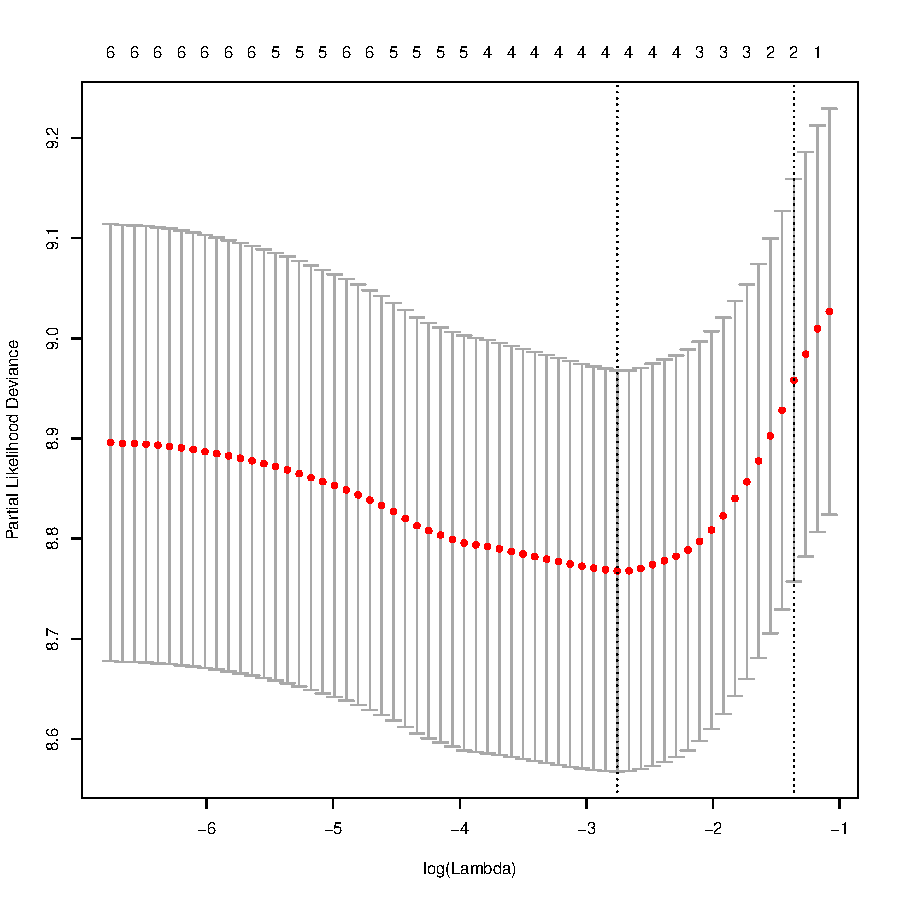
\includegraphics[width=\maxwidth]{figure/nmf-metagene-glmnet-plots-5} 

}


\begin{kframe}\begin{alltt}
\hlkwd{plot}\hlstd{(glmnet.fit.cv.recr_dsd}\hlopt{$}\hlstd{glmnet.fit,} \hlkwc{label} \hlstd{=} \hlnum{TRUE}\hlstd{)}
\hlkwd{abline}\hlstd{(}\hlkwc{v} \hlstd{=} \hlkwd{sum}\hlstd{(}\hlkwd{abs}\hlstd{(}\hlkwd{coef}\hlstd{(glmnet.fit.cv.recr_dsd}\hlopt{$}\hlstd{glmnet.fit,} \hlkwc{s} \hlstd{= glmnet.fit.cv.recr_dsd}\hlopt{$}\hlstd{lambda.1se))))}
\end{alltt}
\end{kframe}

{\centering 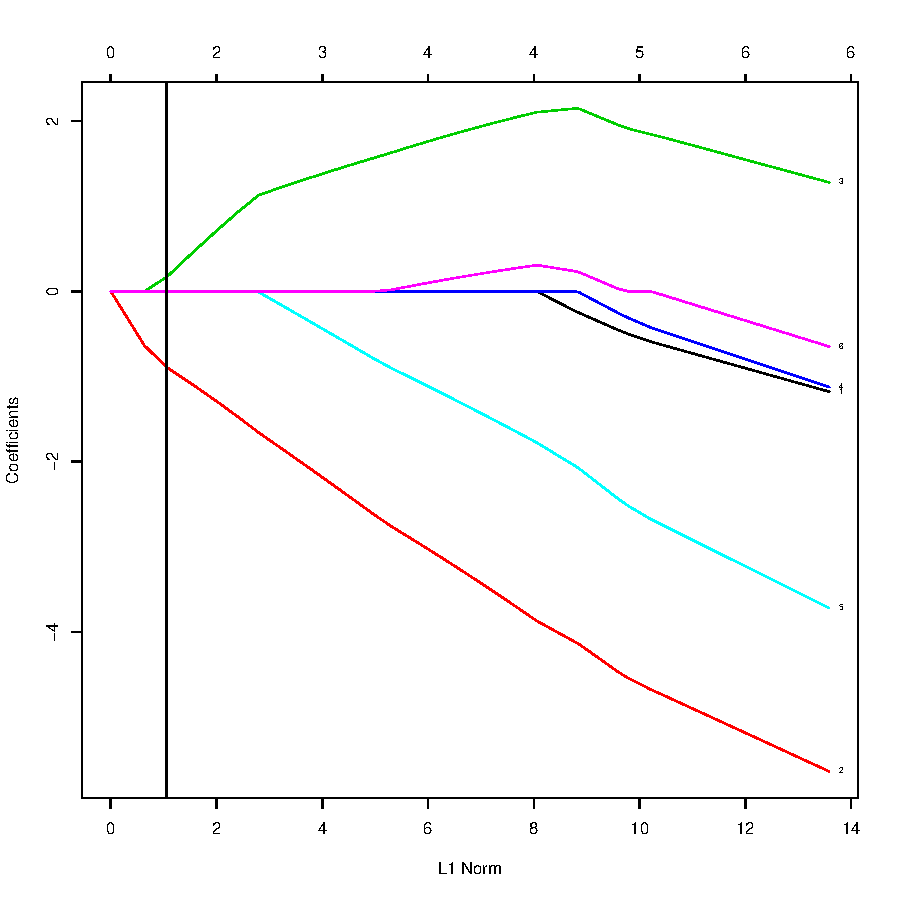
\includegraphics[width=\maxwidth]{figure/nmf-metagene-glmnet-plots-6} 

}


\begin{kframe}\begin{alltt}
\hlcom{#abline(v = sum(abs(coef(glmnet.fit.cv.recr_dsd$glmnet.fit, s = glmnet.fit.cv.recr_dsd$lambda.min))))}
\hlkwd{coef}\hlstd{(glmnet.fit.cv.recr_dsd}\hlopt{$}\hlstd{glmnet.fit,} \hlkwc{s} \hlstd{= glmnet.fit.cv.recr_dsd}\hlopt{$}\hlstd{lambda.1se)}
\end{alltt}
\begin{verbatim}
## 6 x 1 sparse Matrix of class "dgCMatrix"
##          1
## V1  .     
## V2 -1.8877
## V3  1.2420
## V4  .     
## V5 -0.1974
## V6  .
\end{verbatim}
\end{kframe}
\end{knitrout}


%%%%%%%%%%%%%%%%%%%%%%%%%%%%%%%%%%%%%%%%%%%%%%%%%%%%%%%%%%%%%%%%%%%%%%
% SIGNATURE PROGNOSTIC PERFORMANCE: CROSS-VALIDATION
%%%%%%%%%%%%%%%%%%%%%%%%%%%%%%%%%%%%%%%%%%%%%%%%%%%%%%%%%%%%%%%%%%%%%%
% \subsection{Prediction on 10-fold CV}
% <<cv-sig-load>>=
% cv_preds = readRDS("../../analysis/14_SIS_NMF_CV_results.rds")
% @

% <<cv-sig-test-alone>>=
% summary(coxph(y.diag_dsd ~ cv_preds["lasso.1se",]))
% @


%%%%%%%%%%%%%%%%%%%%%%%%%%%%%%%%%%%%%%%%%%%%%%%%%%%%%%%%%%%%%%%%%%%%%%
% SIGNATURE PROGNOSTIC PERFORMANCE: EXTERNAL VALIDATION
%%%%%%%%%%%%%%%%%%%%%%%%%%%%%%%%%%%%%%%%%%%%%%%%%%%%%%%%%%%%%%%%%%%%%%
\subsection{Prediction on validation sets}
\begin{knitrout}
\definecolor{shadecolor}{rgb}{0.969, 0.969, 0.969}\color{fgcolor}\begin{kframe}
\begin{alltt}
\hlkwd{load}\hlstd{(}\hlstr{"../../data/15_validation.rda"}\hlstd{)}
\end{alltt}
\end{kframe}
\end{knitrout}

\begin{knitrout}
\definecolor{shadecolor}{rgb}{0.969, 0.969, 0.969}\color{fgcolor}\begin{kframe}
\begin{alltt}
\hlstd{val.basis} \hlkwb{=} \hlkwd{basis}\hlstd{(nmf.final)}
\hlkwd{rownames}\hlstd{(GSE21501.lingex)} \hlkwb{=} \hlstd{GSE21501.feat}\hlopt{$}\hlstd{Gene.symbol}
\hlkwd{rownames}\hlstd{(GSE28735.lingex)} \hlkwb{=} \hlstd{GSE28735.feat}\hlopt{$}\hlstd{Gene.symbol}
\hlstd{GSE21501.lingex.for_basis} \hlkwb{=} \hlstd{GSE21501.lingex[}\hlkwd{match}\hlstd{(}\hlkwd{rownames}\hlstd{(val.basis),} \hlkwd{rownames}\hlstd{(GSE21501.lingex)),]}
\hlstd{GSE28735.lingex.for_basis} \hlkwb{=} \hlstd{GSE28735.lingex[}\hlkwd{match}\hlstd{(}\hlkwd{rownames}\hlstd{(val.basis),} \hlkwd{rownames}\hlstd{(GSE28735.lingex)),]}
\hlstd{GSE21501.lingex.for_basis[}\hlkwd{is.na}\hlstd{(GSE21501.lingex.for_basis)]} \hlkwb{=} \hlnum{0}
\hlstd{GSE28735.lingex.for_basis[}\hlkwd{is.na}\hlstd{(GSE28735.lingex.for_basis)]} \hlkwb{=} \hlnum{0}

\hlstd{GSE21501.coefs} \hlkwb{=} \hlkwd{apply}\hlstd{(GSE21501.lingex.for_basis,} \hlnum{2}\hlstd{,} \hlkwa{function}\hlstd{(}\hlkwc{xcol}\hlstd{)} \hlkwd{nnls}\hlstd{(val.basis, xcol)}\hlopt{$}\hlstd{x)}
\hlstd{GSE28735.coefs} \hlkwb{=} \hlkwd{apply}\hlstd{(GSE28735.lingex.for_basis,} \hlnum{2}\hlstd{,} \hlkwa{function}\hlstd{(}\hlkwc{xcol}\hlstd{)} \hlkwd{nnls}\hlstd{(val.basis, xcol)}\hlopt{$}\hlstd{x)}

\hlstd{GSE21501.axis1} \hlkwb{=} \hlstd{GSE21501.coefs[}\hlnum{1}\hlstd{,]} \hlopt{-} \hlstd{GSE21501.coefs[}\hlnum{5}\hlstd{,]}
\hlstd{GSE21501.axis2} \hlkwb{=} \hlstd{GSE21501.coefs[}\hlnum{6}\hlstd{,]} \hlopt{-} \hlstd{GSE21501.coefs[}\hlnum{2}\hlstd{,]}
\hlstd{GSE28735.axis1} \hlkwb{=} \hlstd{GSE28735.coefs[}\hlnum{1}\hlstd{,]} \hlopt{-} \hlstd{GSE28735.coefs[}\hlnum{5}\hlstd{,]}
\hlstd{GSE28735.axis2} \hlkwb{=} \hlstd{GSE28735.coefs[}\hlnum{6}\hlstd{,]} \hlopt{-} \hlstd{GSE28735.coefs[}\hlnum{2}\hlstd{,]}

\hlstd{GSE21501.score} \hlkwb{=} \hlnum{1.354}\hlopt{*}\hlstd{GSE21501.axis1} \hlopt{+} \hlnum{1.548}\hlopt{*}\hlstd{GSE21501.axis2}
\hlstd{GSE28735.score} \hlkwb{=} \hlnum{1.354}\hlopt{*}\hlstd{GSE28735.axis1} \hlopt{+} \hlnum{1.548}\hlopt{*}\hlstd{GSE28735.axis2}

\hlstd{GSE21501.pcna} \hlkwb{=} \hlkwd{apply}\hlstd{(GSE21501.gex[}\hlkwd{match}\hlstd{(metapcna.sig, GSE21501.feat}\hlopt{$}\hlstd{Gene.symbol),],} \hlnum{2}\hlstd{, median,} \hlkwc{na.rm} \hlstd{=} \hlnum{TRUE}\hlstd{)}
\hlstd{GSE28735.pcna} \hlkwb{=} \hlkwd{apply}\hlstd{(GSE28735.gex[}\hlkwd{match}\hlstd{(metapcna.sig, GSE28735.feat}\hlopt{$}\hlstd{Gene.symbol),],} \hlnum{2}\hlstd{, median,} \hlkwc{na.rm} \hlstd{=} \hlnum{TRUE}\hlstd{)}
\end{alltt}
\end{kframe}
\end{knitrout}

\begin{knitrout}
\definecolor{shadecolor}{rgb}{0.969, 0.969, 0.969}\color{fgcolor}\begin{kframe}
\begin{alltt}
\hlstd{temp} \hlkwb{=} \hlkwd{coxph}\hlstd{(}\hlkwd{Surv}\hlstd{(GSE21501.samp}\hlopt{$}\hlstd{time, GSE21501.samp}\hlopt{$}\hlstd{event)} \hlopt{~} \hlstd{GSE21501.score)}
\hlkwd{summary}\hlstd{(temp)}
\end{alltt}
\begin{verbatim}
## Call:
## coxph(formula = Surv(GSE21501.samp$time, GSE21501.samp$event) ~ 
##     GSE21501.score)
## 
##   n= 102, number of events= 66 
## 
##                coef exp(coef) se(coef)    z Pr(>|z|)
## GSE21501.score 1.81      6.13     1.14 1.59     0.11
## 
##                exp(coef) exp(-coef) lower .95 upper .95
## GSE21501.score      6.13      0.163     0.655      57.3
## 
## Concordance= 0.577  (se = 0.042 )
## Rsquare= 0.024   (max possible= 0.993 )
## Likelihood ratio test= 2.49  on 1 df,   p=0.115
## Wald test            = 2.52  on 1 df,   p=0.112
## Score (logrank) test = 2.54  on 1 df,   p=0.111
\end{verbatim}
\begin{alltt}
\hlstd{temp} \hlkwb{=} \hlkwd{coxph}\hlstd{(}\hlkwd{Surv}\hlstd{(GSE28735.samp}\hlopt{$}\hlstd{time, GSE28735.samp}\hlopt{$}\hlstd{event)} \hlopt{~} \hlstd{GSE28735.score)}
\hlkwd{summary}\hlstd{(temp)}
\end{alltt}
\begin{verbatim}
## Call:
## coxph(formula = Surv(GSE28735.samp$time, GSE28735.samp$event) ~ 
##     GSE28735.score)
## 
##   n= 42, number of events= 29 
## 
##                 coef exp(coef) se(coef)    z Pr(>|z|)
## GSE28735.score 1.867     6.471    0.752 2.48    0.013
## 
##                exp(coef) exp(-coef) lower .95 upper .95
## GSE28735.score      6.47      0.155      1.48      28.2
## 
## Concordance= 0.655  (se = 0.064 )
## Rsquare= 0.132   (max possible= 0.981 )
## Likelihood ratio test= 5.92  on 1 df,   p=0.0149
## Wald test            = 6.17  on 1 df,   p=0.013
## Score (logrank) test = 6.46  on 1 df,   p=0.011
\end{verbatim}
\begin{alltt}
\hlkwd{anova}\hlstd{(}\hlkwd{coxph}\hlstd{(}\hlkwd{Surv}\hlstd{(GSE21501.samp}\hlopt{$}\hlstd{time, GSE21501.samp}\hlopt{$}\hlstd{event)} \hlopt{~} \hlstd{GSE21501.axis1} \hlopt{+} \hlstd{GSE21501.axis2))}
\end{alltt}
\begin{verbatim}
## Analysis of Deviance Table
##  Cox model: response is Surv(GSE21501.samp$time, GSE21501.samp$event)
## Terms added sequentially (first to last)
## 
##                loglik Chisq Df Pr(>|Chi|)
## NULL             -255                    
## GSE21501.axis1   -254  1.44  1       0.23
## GSE21501.axis2   -254  1.09  1       0.30
\end{verbatim}
\begin{alltt}
\hlkwd{anova}\hlstd{(}\hlkwd{coxph}\hlstd{(}\hlkwd{Surv}\hlstd{(GSE28735.samp}\hlopt{$}\hlstd{time, GSE28735.samp}\hlopt{$}\hlstd{event)} \hlopt{~} \hlstd{GSE28735.axis1} \hlopt{+} \hlstd{GSE28735.axis2))}
\end{alltt}
\begin{verbatim}
## Analysis of Deviance Table
##  Cox model: response is Surv(GSE28735.samp$time, GSE28735.samp$event)
## Terms added sequentially (first to last)
## 
##                loglik Chisq Df Pr(>|Chi|)
## NULL            -83.1                    
## GSE28735.axis1  -81.4  3.43  1      0.064
## GSE28735.axis2  -80.2  2.51  1      0.113
\end{verbatim}
\end{kframe}
\end{knitrout}
















